%%%%%%%%%%%%%%%%%%%%%%%%%%%%%%%%%%%%%%%%%
% KOMA-Script Presentation
% LaTeX Template
% Version 1.0 (3/3/13)
%
% This template has been downloaded from:
% http://www.LaTeXTemplates.com
%
% Original Authors:
% Marius Hofert (marius.hofert@math.ethz.ch)
% Markus Kohm (komascript@gmx.info)
% Described in the PracTeX Journal, 2010, No. 2
%
% License:
% CC BY-NC-SA 3.0 (http://creativecommons.org/licenses/by-nc-sa/3.0/)
%
%%%%%%%%%%%%%%%%%%%%%%%%%%%%%%%%%%%%%%%%%

%----------------------------------------------------------------------------------------
%	PACKAGES AND OTHER DOCUMENT CONFIGURATIONS
%----------------------------------------------------------------------------------------

\documentclass[
paper=128mm:96mm, % The same paper size as used in the beamer class
fontsize=11pt, % Font size
pagesize, % Write page size to dvi or pdf
parskip=half-, % Paragraphs separated by half a line
]{scrartcl} % KOMA script (article)

\linespread{1.12} % Increase line spacing for readability

%------------------------------------------------
% Colors
\usepackage{xcolor}	 % Required for custom colors
% Define a few colors for making text stand out within the presentation
\definecolor{mygreen}{RGB}{44,85,17}
\definecolor{myblue}{RGB}{34,31,217}
\definecolor{mybrown}{RGB}{194,164,113}
\definecolor{myred}{RGB}{255,66,56}
\definecolor{myyellow}{RGB}{236,232,37}
% Use these colors within the presentation by enclosing text in the commands below
\newcommand*{\mygreen}[1]{\textcolor{mygreen}{#1}}
\newcommand*{\myblue}[1]{\textcolor{myblue}{#1}}
\newcommand*{\mybrown}[1]{\textcolor{mybrown}{#1}}
\newcommand*{\myred}[1]{\textcolor{myred}{#1}}
\newcommand*{\myyellow}[1]{\textcolor{myyelow}{#1}}
%------------------------------------------------

%------------------------------------------------
% Margins
\usepackage[ % Page margins settings
includeheadfoot,
top=3.5mm,
bottom=3.5mm,
left=5.5mm,
right=5.5mm,
headsep=6.5mm,
foot skip=8.5mm
]{geometry}
%------------------------------------------------

%------------------------------------------------
% % Fonts
% \usepackage[T1]{fontenc}	 % For correct hyphenation and T1 encoding
% \usepackage{lmodern} % Default font: latin modern font
% %\usepackage{fourier} % Alternative font: utopia
% %\usepackage{charter} % Alternative font: low-resolution roman font
% \renewcommand{\familydefault}{\sfdefault} % Sans serif - this may need to be commented to see the alternative fonts

% ========================
% fbb Bembo package
% \usepackage[full]{textcomp} % to get the right copyright, etc.
\usepackage[lining,tabular]{fbb} % so math uses tabular lining figures
\usepackage[scaled=.95,type1]{cabin} % sans serif in style of Gill Sans
\usepackage[varqu,varl]{zi4}% inconsolata typewriter
% \usepackage[T1]{fontenc} % LY1 also works
\usepackage[utf8]{inputenc}
% \usepackage[libertine,bigdelims]{newtxmath}
\usepackage[cal=boondoxo,bb=boondox,frak=boondox]{mathalfa}
\useosf % change normal text to use proportional oldstyle figures
% \usetosf would provide tabular oldstyle figures in text
% ========================

%------------------------------------------------

%------------------------------------------------
% Various required packages
\usepackage{amsthm} % Required for theorem environments
\usepackage{bm} % Required for bold math symbols (used in the footer of the slides)
\usepackage{graphicx} % Required for including images in figures
\graphicspath{{img/}} % Sets the default location of pictures
\usepackage{tikz} % Required for colored boxes
\usepackage{booktabs} % Required for horizontal rules in tables
\usepackage{multicol} % Required for creating multiple columns in slides
\usepackage{lastpage} % For printing the total number of pages at the
                      % bottom of each slide
\usepackage[english]{babel} % Document language - required for
                            % customizing section titles
\usepackage{microtype} % Better typography
\usepackage{tocstyle} % Required for customizing the table of contents
%------------------------------------------------

%------------------------------------------------
% Slide layout configuration
\usepackage{scrpage2} % Required for customization of the header and footer
\pagestyle{scrheadings} % Activates the pagestyle from scrpage2 for custom headers and footers
\clearscrheadfoot % Remove the default header and footer
\setkomafont{pageheadfoot}{\normalfont\color{black}\sffamily} % Font settings for the header and footer

% Sets vertical centering of slide contents with increased space between paragraphs/lists
\makeatletter
\renewcommand*{\@textbottom}{\vskip \z@ \@plus 1fil}
\newcommand*{\@texttop}{\vskip \z@ \@plus .5fil}
\addtolength{\parskip}{\z@\@plus .25fil}
\makeatother

% Remove page numbers and the dots leading to them from the outline slide
\makeatletter
\newtocstyle[noonewithdot]{nodotnopagenumber}{\settocfeature{pagenumberbox}{\@gobble}}
\makeatother
\usetocstyle{nodotnopagenumber}

\AtBeginDocument{\renewcaptionname{english}{\contentsname}{\Large Outline}} % Change the name of the table of contents
%------------------------------------------------

%------------------------------------------------
% Header configuration - if you don't want a header remove this block
\ihead{
\hspace{-2mm}
\begin{tikzpicture}[remember picture,overlay]
\node [xshift=\paperwidth/2,yshift=-\headheight] (mybar) at (current page.north west)[rectangle,fill,inner sep=0pt,minimum width=\paperwidth,minimum height=2\headheight,top color=mygreen!64,bottom color=mygreen]{}; % Colored bar
\node[below of=mybar,yshift=3.3mm,rectangle,shade,inner sep=0pt,minimum width=128mm,minimum height =1.5mm,top color=black!50,bottom color=white]{}; % Shadow under the colored bar
shadow
\end{tikzpicture}
\color{white}\runninghead} % Header text defined by the \runninghead
                           % command below and colored white for
                           % contrast

%------------------------------------------------

%------------------------------------------------
% Footer configuration
%\newlength{\footheight}
\setlength{\footheight}{8mm} % Height of the footer
% \addtokomafont{pagefoot}{\footnotesize} % Small font size for the footnote
\addtokomafont{pagefoot}{\tiny}

\ifoot{% Left side
\hspace{-2mm}
\begin{tikzpicture}[remember picture,overlay]
\node [xshift=\paperwidth/2,yshift=\footheight] at (current page.south west)[rectangle,fill,inner sep=0pt,minimum width=\paperwidth,minimum height=3pt,top color=mygreen,bottom color=mygreen]{}; % Green bar
\end{tikzpicture}
\myauthor\ \raisebox{0.2mm}{$\bm{\vert}$}\ \myuni % Left side text
}

\ofoot[\pagemark/\pageref{LastPage}\hspace{-2mm}]{\pagemark/\pageref{LastPage}\hspace{-2mm}} % Right side
%------------------------------------------------

%------------------------------------------------
% Section spacing - deeper section titles are given less space due to lesser importance
\usepackage{titlesec} % Required for customizing section spacing
\titlespacing{\section}{0mm}{0mm}{0mm} % Lengths are: left, before, after
\titlespacing{\subsection}{0mm}{0mm}{-1mm} % Lengths are: left, before, after
\titlespacing{\subsubsection}{0mm}{0mm}{-2mm} % Lengths are: left, before, after
\setcounter{secnumdepth}{0} % How deep sections are numbered, set to no numbering by default - change to 1 for numbering sections, 2 for numbering sections and subsections, etc
%------------------------------------------------

%------------------------------------------------
% Theorem style
\newtheoremstyle{mythmstyle} % Defines a new theorem style used in this template
{0.5em} % Space above
{0.5em} % Space below
{} % Body font
{} % Indent amount
{\sffamily\bfseries} % Head font
{} % Punctuation after head
{\newline} % Space after head
{\thmname{#1}\ \thmnote{(#3)}} % Head spec

\theoremstyle{mythmstyle} % Change the default style of the theorem to the one defined above
\newtheorem{theorem}{Theorem}[section] % Label for theorems
\newtheorem{remark}[theorem]{Remark} % Label for remarks
\newtheorem{algorithm}[theorem]{Algorithm} % Label for algorithms
\makeatletter % Correct qed adjustment
%------------------------------------------------

%------------------------------------------------
% The code for the box which can be used to highlight an element of a slide (such as a theorem)
\newcommand*{\mybox}[2]{ % The box takes two arguments: width and content
\par\noindent
\begin{tikzpicture}[mynodestyle/.style={rectangle,draw=mygreen,thick,inner sep=2mm,text justified,top color=white,bottom color=white,above}]\node[mynodestyle,at={(0.5*#1+2mm+0.4pt,0)}]{ % Box formatting
\begin{minipage}[t]{#1}
#2
\end{minipage}
};
\end{tikzpicture}
\par\vspace{-1.3em}}
%------------------------------------------------

%----------------------------------------------------------------------------------------
%	PRESENTATION INFORMATION
%----------------------------------------------------------------------------------------

\newcommand*{\mytitle}{Solicitud de Ingreso. Tesis de Maestría.} % Title
\newcommand*{\runninghead}{Solicitud de Ingreso al Doctorado en Nanociencias y Nanotecnología} % Running head displayed on
                                % almost all slides
\newcommand*{\myauthor}{Sergio-Feliciano Mendoza-Barrera} % Presenters name(s)
\newcommand*{\mydate}{Julio 29, 2014} % Presentation date
\newcommand*{\myuni}{smendoza.barrera@globallabs.org} % University or department

%----------------------------------------------------------------------------------------

\begin{document}

%----------------------------------------------------------------------------------------
%	TITLE SLIDE
%----------------------------------------------------------------------------------------

% Title slide - you may have to tweak a few of the numbers if you wish to make changes to the layout
\thispagestyle{empty} % No slide header and footer
\begin{tikzpicture}[remember picture,overlay] % Background box
\node [xshift=\paperwidth/2,yshift=\paperheight/2] at (current page.south west)[rectangle,fill,inner sep=0pt,minimum width=\paperwidth,minimum height=\paperheight/3,top color=mygreen,bottom color=mygreen]{}; % Change the height of the box, its colors and position on the page here
\end{tikzpicture}
% Text within the box
\begin{flushright}
\vspace{0.6cm}
\color{white}\sffamily
{\bfseries\Large\mytitle\par} % Title
\vspace{0.5cm}
\normalsize
\myauthor\par % Author name
\mydate\par % Date
\vfill
\end{flushright}

\clearpage

%----------------------------------------------------------------------------------------
%	TABLE OF CONTENTS
%----------------------------------------------------------------------------------------

\thispagestyle{empty} % No slide header and footer

\small\tableofcontents % Change the font size and print the table of contents - it may be useful to shrink the font size further if the presentation is full of sections
% To exclude sections/subsections from the table of contents, put an asterisk after \(sub)section like so: \section*{Section Name}

\clearpage

%----------------------------------------------------------------------------------------
%	PRESENTATION SLIDES
%----------------------------------------------------------------------------------------

\section{Datos de la Tesis de Maestría}

\textbf{``Pruebas de CI's aplicando un pulso en las Fuentes de Polarización''}

   Por:

   \textbf{Sergio-Feliciano Mendoza-Barrera}

   Supervisada por:

   \textit{Dr. Víctor Champac-Vilela}

   \textit{Dr. Mónico Linares-Aranda}

\clearpage

%------------------------------------------------

\subsection{Estado del Arte (2000): Defectos en CI's}

\begin{multicols}{2} % Divide text into multiple columns
\begin{itemize}
  \item Corto-circuitos entre\\conductores
  \item Roturas en los conductores
  \item Roturas en los contactos o vías
  \item Uniones P-N defectuosas
\end{itemize}
\end{multicols}

\begin{figure}[h]
\centering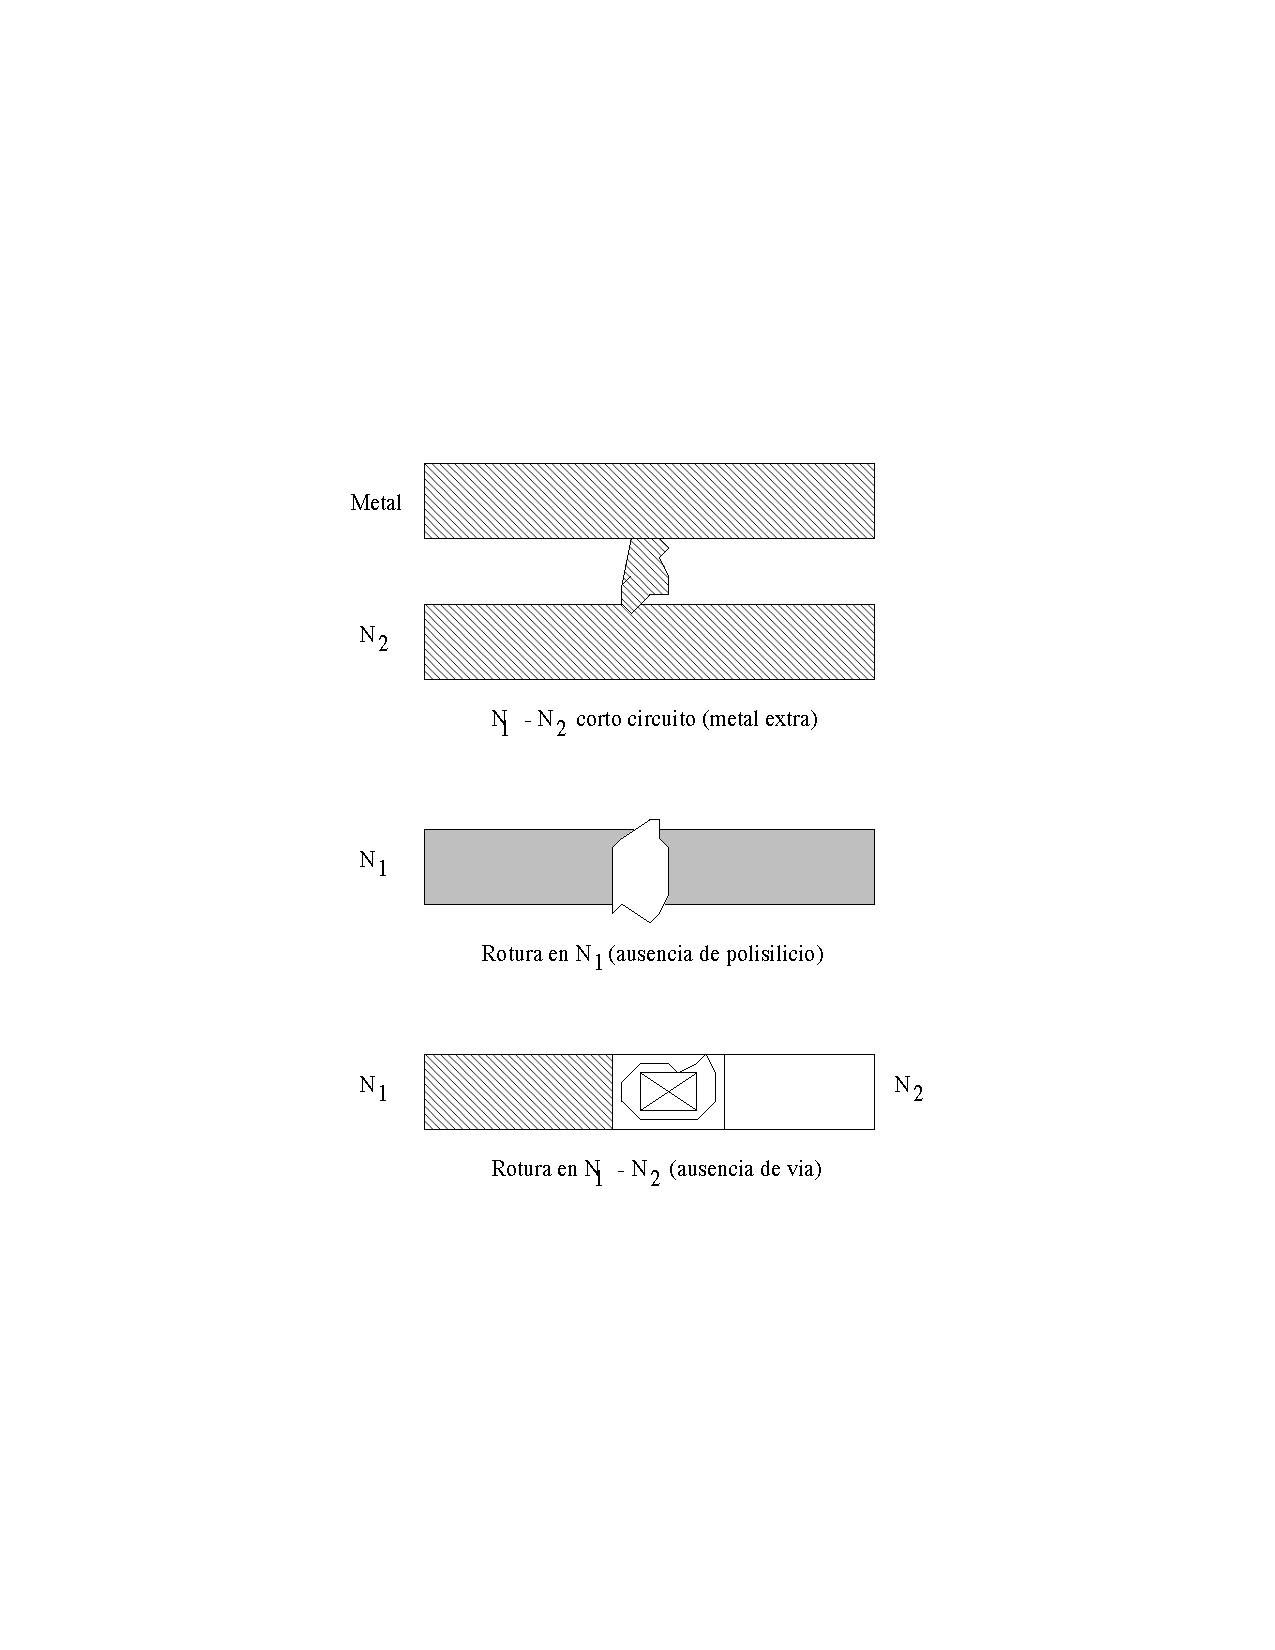
\includegraphics[width=0.23\linewidth]{defectos}
\end{figure}


% \textit{Sed iaculis} dapibus gravida. Morbi sed tortero erat, nec
% interdum arcu. Sed id lorem lectus. Quisque viverra augue id sem
% ornare non aliquam nibh tristique. Aenean in ligula nisl. Nulla sed
% tellus ipsum.

% \begin{multicols}{2} % Divide text into multiple columns
%   \mygreen{Sed diam enim, sagittis nec} condimentum sit amet,
%   ullamcorper sit amet libero. \mybrown{Aliquam vel dui orci}, a porta
%   odio. \myred{Nullam id suscipit} ipsum. \myblue{Aenean lobortis}
%   commodo sem, ut commodo leo gravida vitae. Pellentesque vehicula ante
%   iaculis arcu pretium rutrum eget sit amet purus. Integer ornare nulla
%   quis neque ultrices lobortis. Vestibulum ultrices tincidunt libero,
%   quis commodo erat ullamcorper id.
% \end{multicols}

\clearpage

%------------------------------------------------

\subsection{Pruebas de CI's}

\begin{multicols}{2} % Divide text into multiple columns
  \begin{itemize}
  \item Esquema General de pruebas a CI's
    \begin{itemize}
    \item  Aplicación de vectores de prueba
    \item La medición en un punto observable
    \item Comparación con respecto a la referencia
    \end{itemize}
  \end{itemize}
\end{multicols}

\begin{figure}[h]
\centering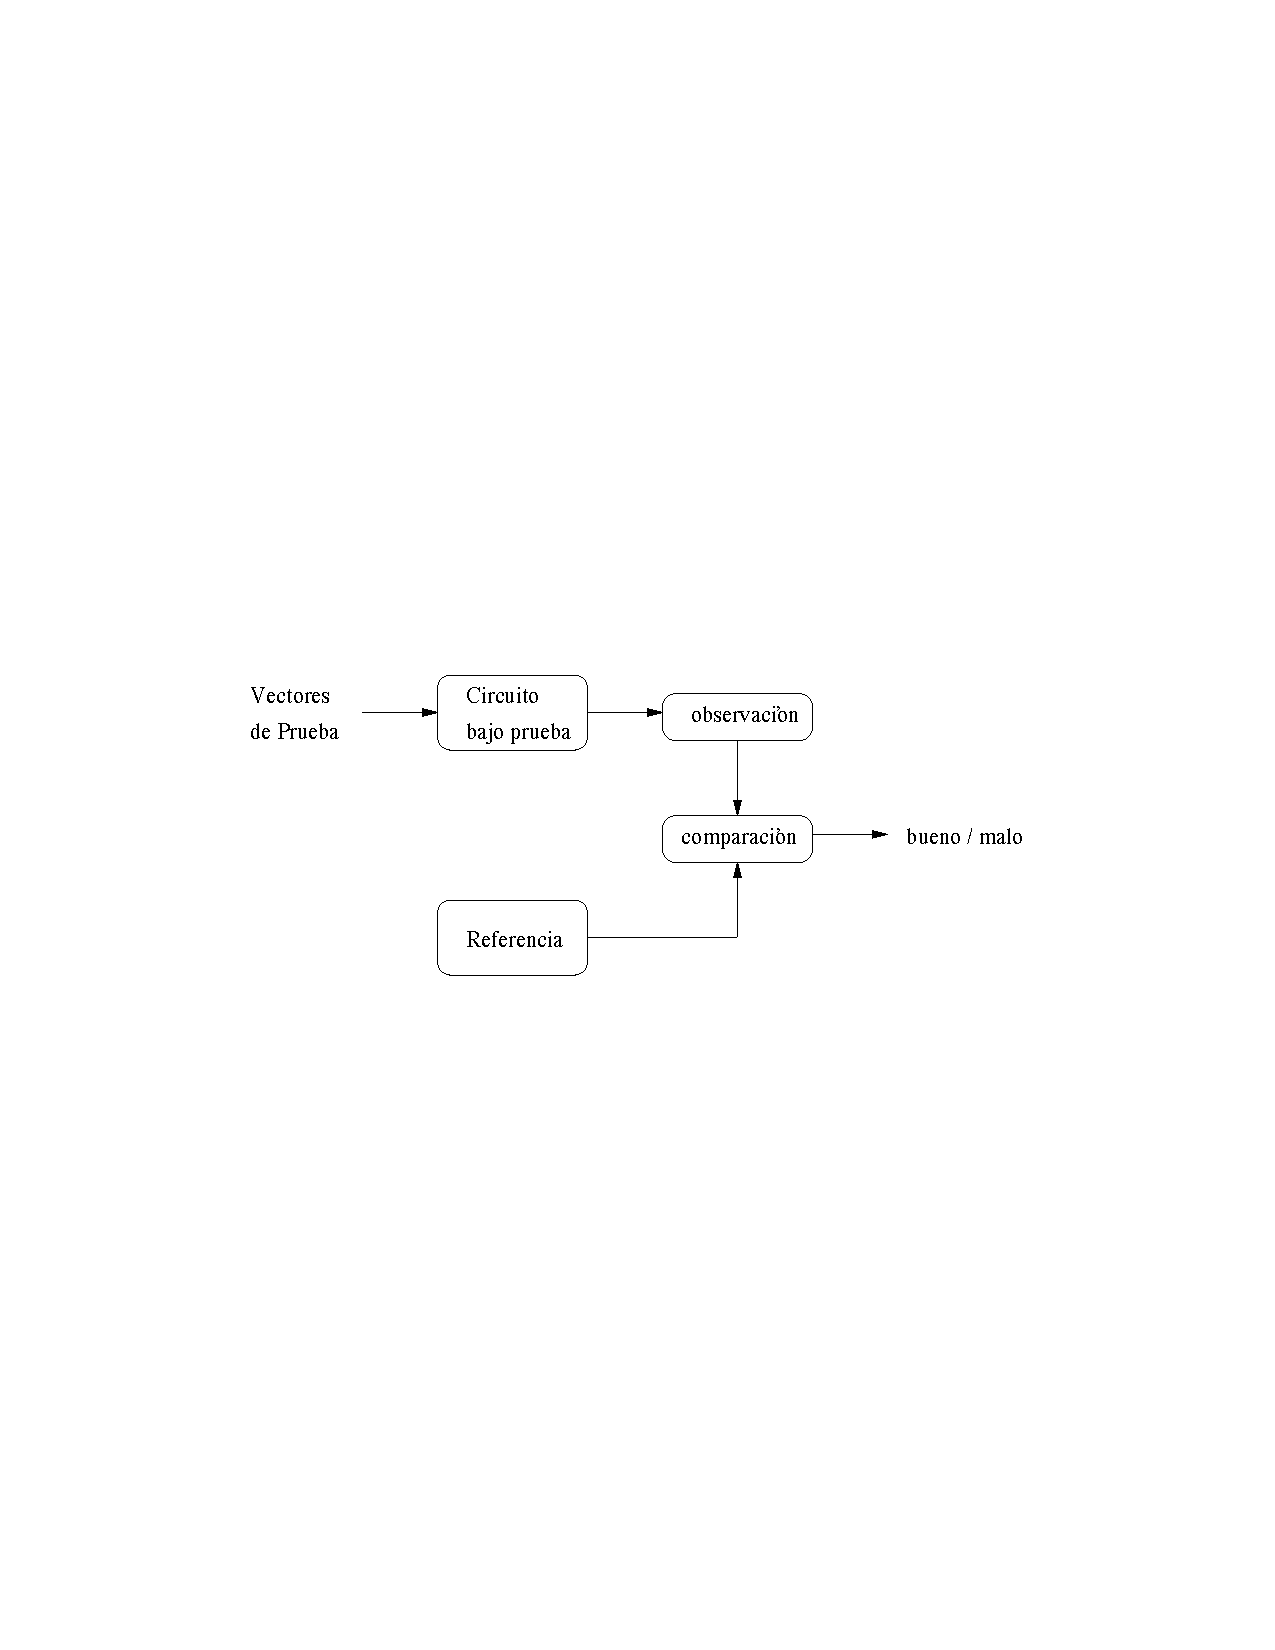
\includegraphics[width=0.6\linewidth]{esquema}
\end{figure}

% \begin{enumerate}
% \item Nulla commodo, erat quis gravida posuere, elit lacus lobortis est, quis porttitor odio mauris at libero
% \item Nam cursus est eget velit posuere pellentesque
% \item Vestibulum faucibus velit a augue condimentum quis convallis nulla gravida
% \end{enumerate}

\clearpage

%------------------------------------------------

\subsection{Modelos de fallas}

\begin{itemize}
\item \textbf{Fallas tipo Stuck-at}
  \begin{itemize}
  \item Un vector puede detectar mas de una falla
  \item Diferentes vectores detectan la misma falla
  \end{itemize}

  \begin{figure}[h]
    \centering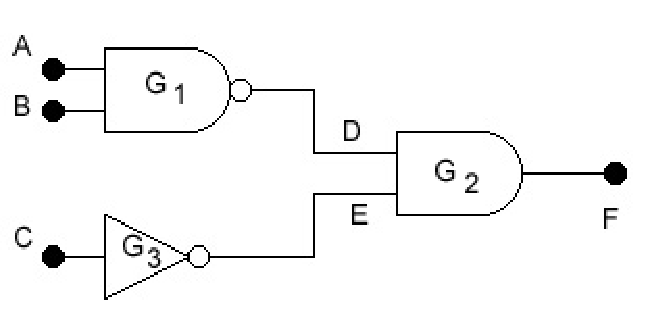
\includegraphics[width=0.5\linewidth]{combina01}
  \end{figure}
  \clearpage

\item \textbf{Fallas Stuck-Open}
  \begin{itemize}
  \item Prueba de doble patrón
  \item Propagación del error
  \item Generación automática de vectores de test
  \end{itemize}

  \begin{figure}[h]
    \centering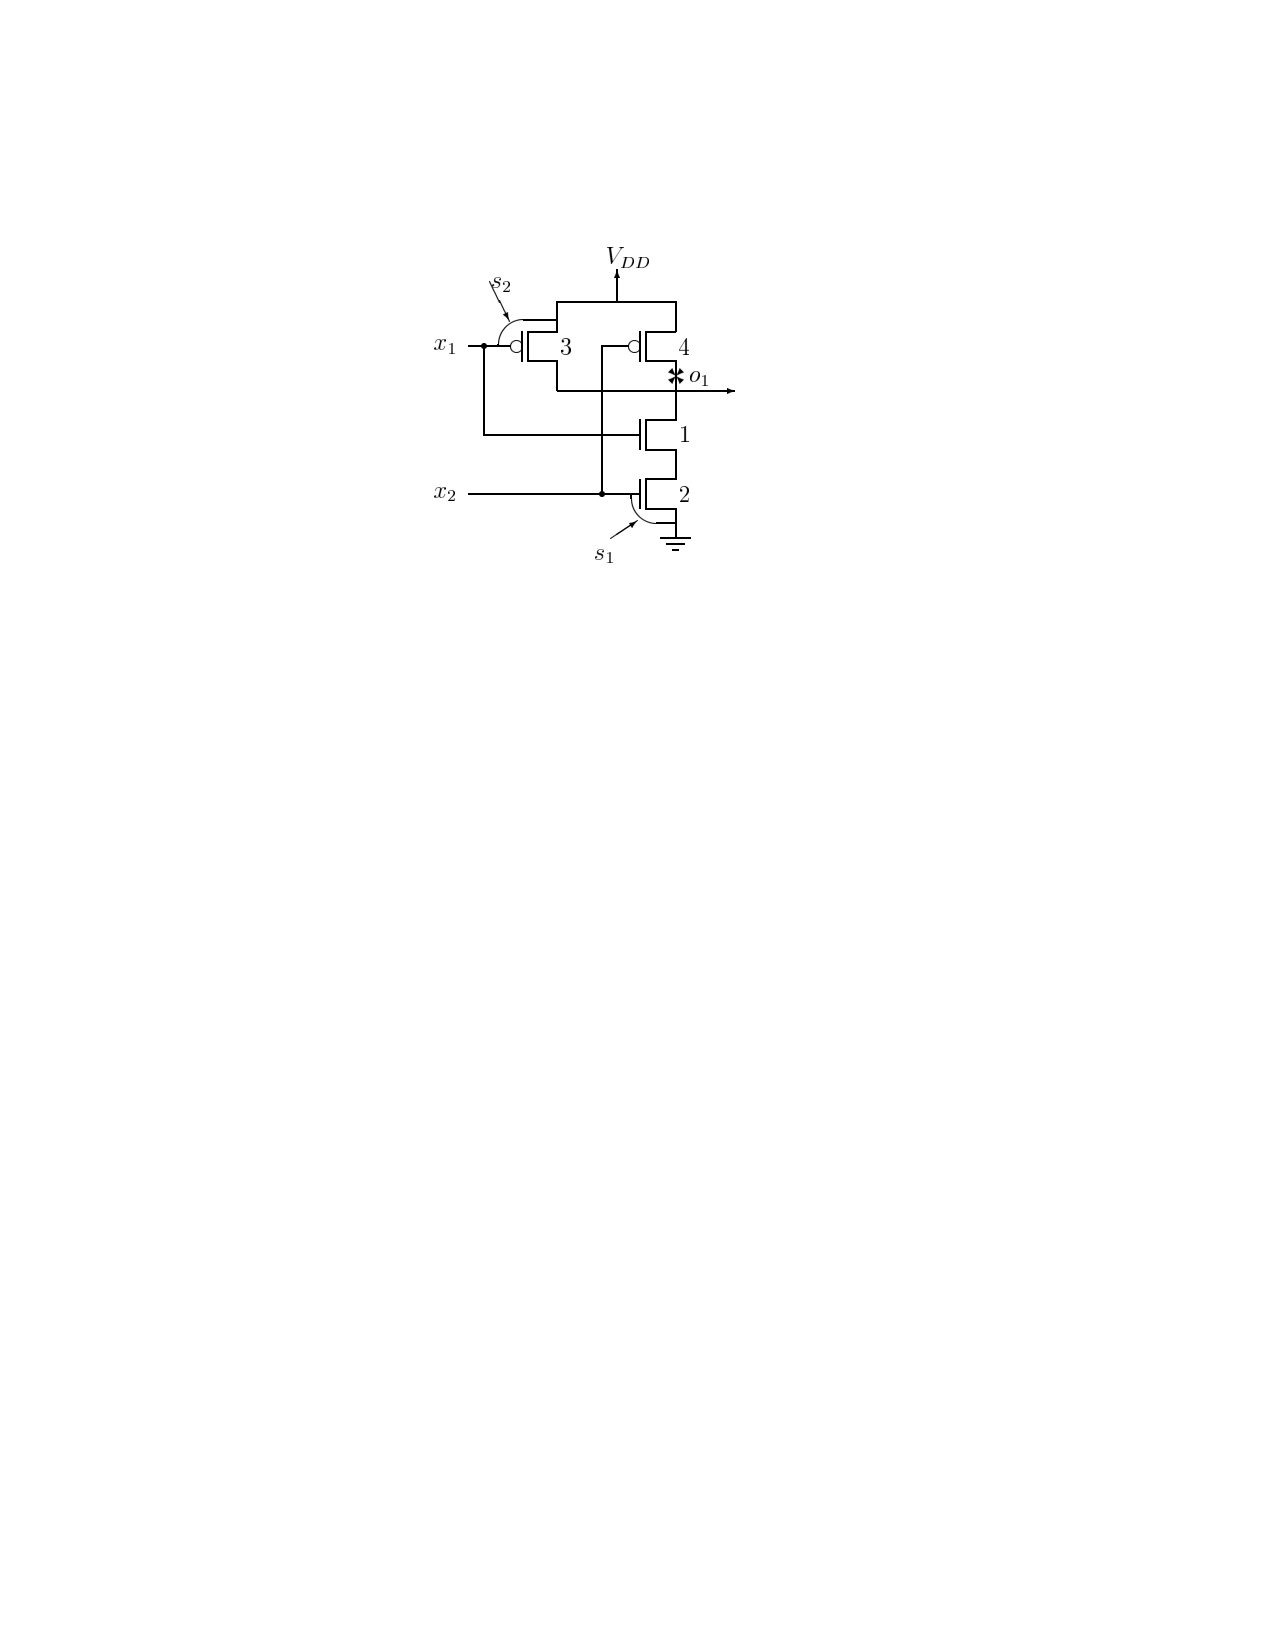
\includegraphics[width=0.5\linewidth]{stuckOpen}
  \end{figure}

\clearpage

\item \textbf{Fallas Stuck-on}

\mybox{0.8\textwidth}{ % Example of encapsulating text in a colored box
% \begin{theorem}[Modelo]
    $$V_f = \frac{R_n}{R_n + 2 R_p} V_{DD}$$
% \end{theorem}
}

\begin{itemize}
\item Algún transistor permanece encendido
\item Selección adecuada de vectores de prueba
\end{itemize}

\begin{figure}[h]
  \centering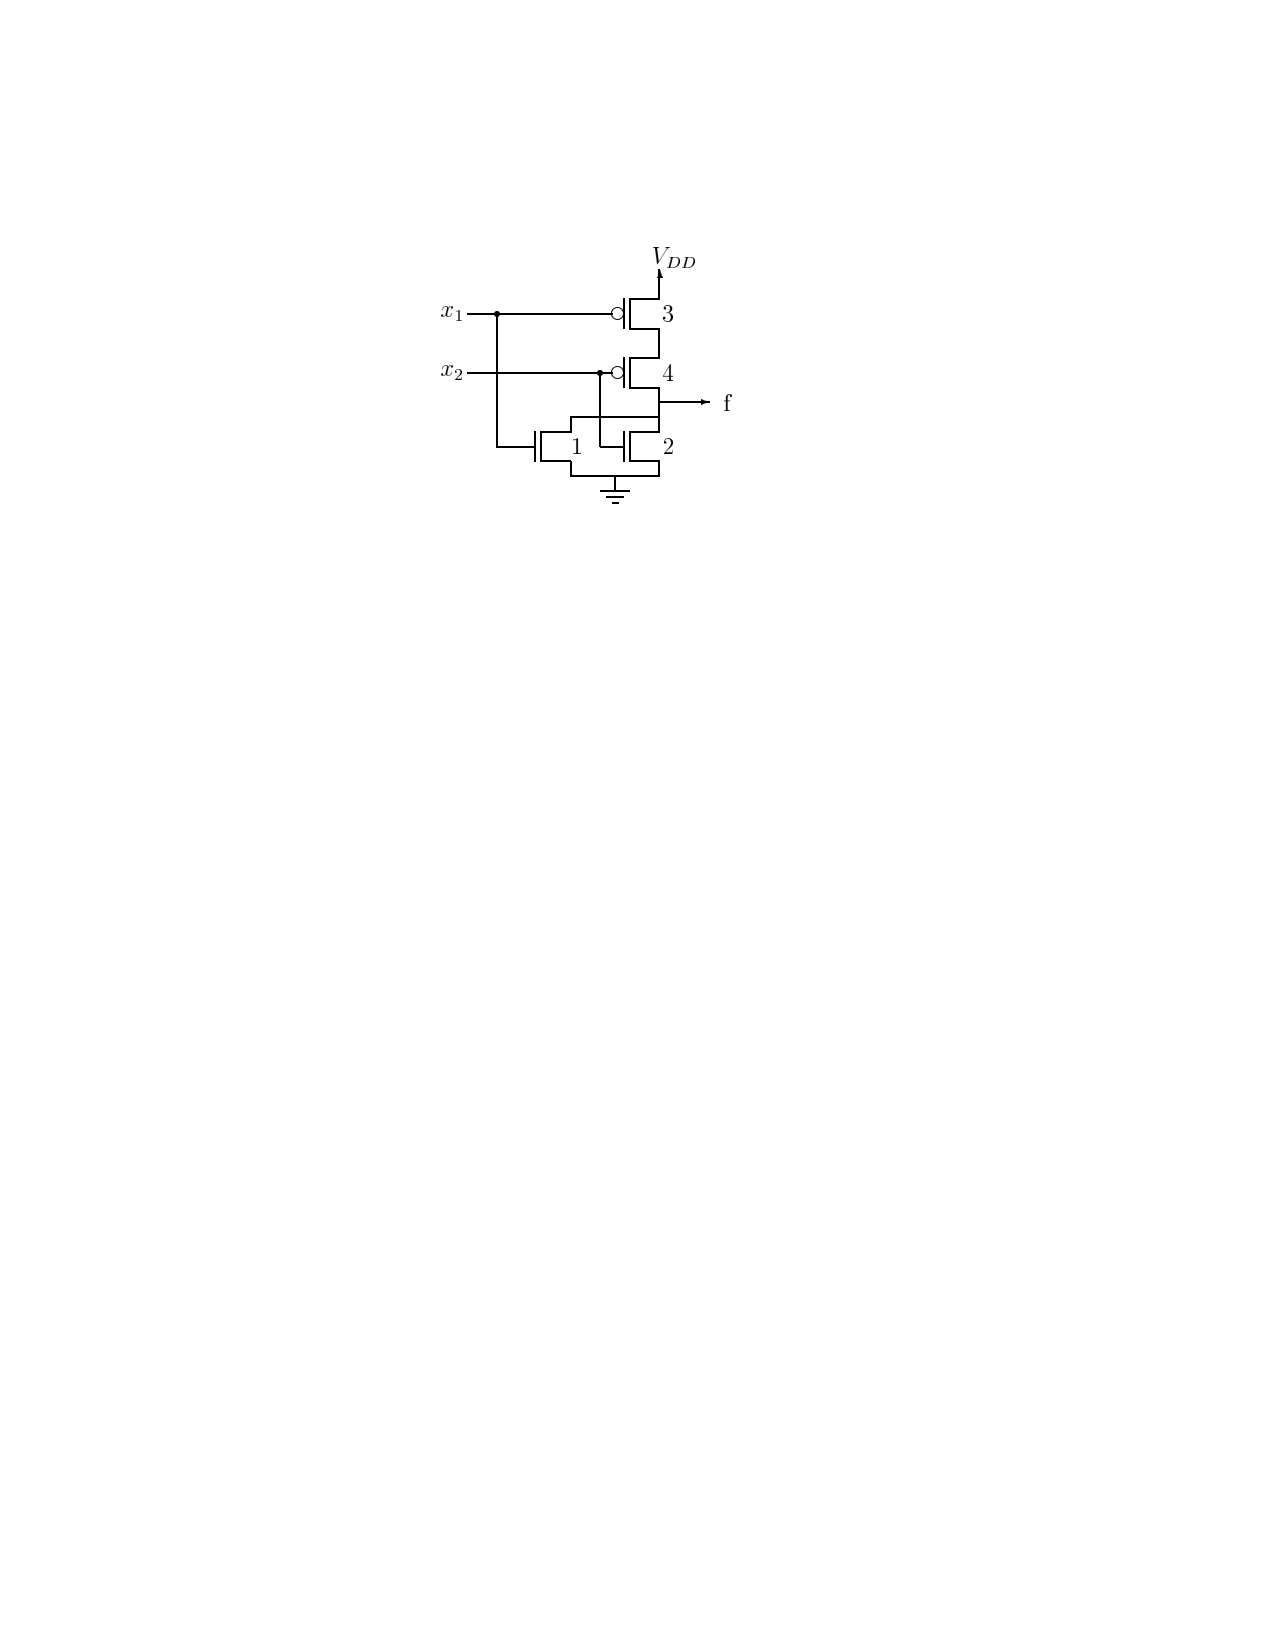
\includegraphics[width=0.5\linewidth]{stuckOn}
\end{figure}

\clearpage

\item \textbf{Fallas de tipo puente o corto circuito}
  \begin{itemize}
  \item Tipo no retroalimentante en un elemento
  \item Tipo no retroalimentante entre dos elementos
  \item Retroalimentante
  \end{itemize}
\end{itemize}

  \begin{figure}[h]
    \centering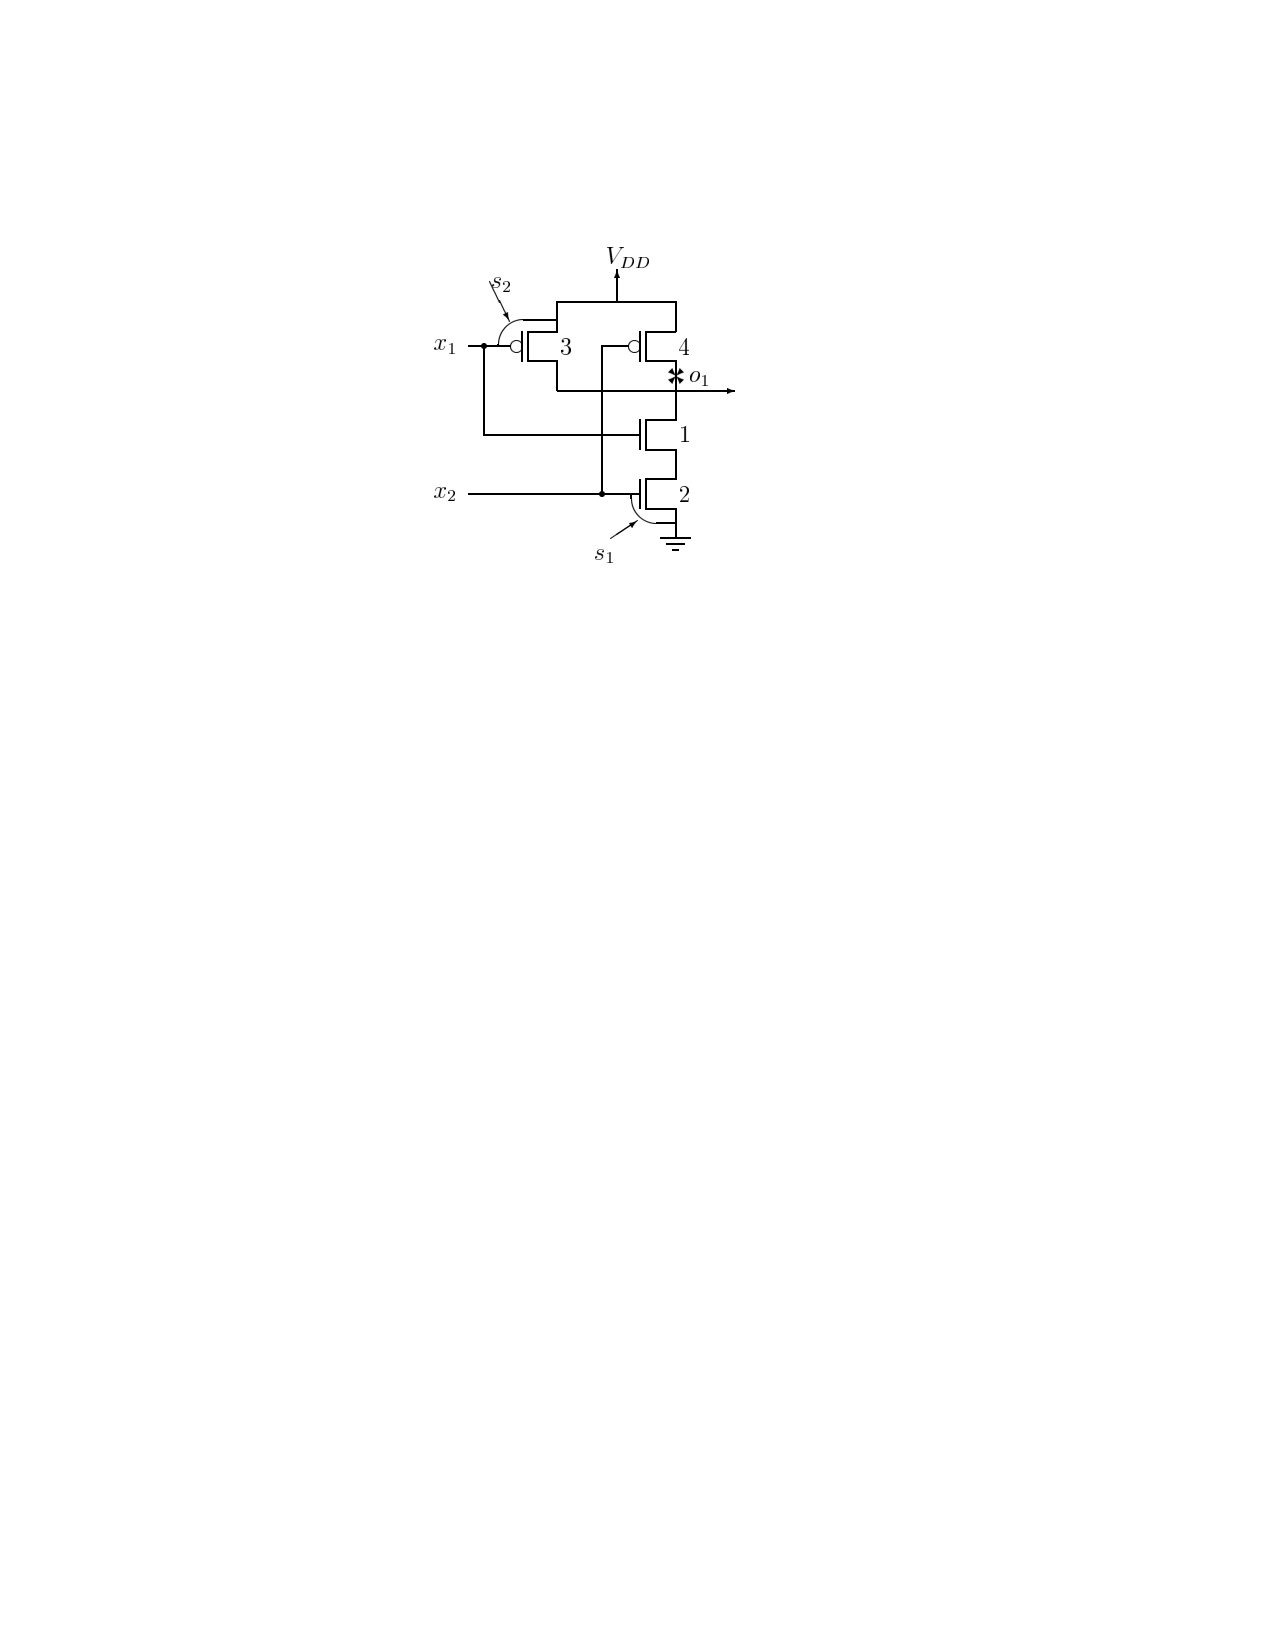
\includegraphics[width=0.5\linewidth]{stuckOpen}
  \end{figure}

% How to include a theorem in this presentation:
% \begin{verbatim}
% \mybox{0.8\textwidth}{
% \begin{theorem}[Murphy (1949)]
% Anything that can go wrong, will go wrong.
% \end{theorem}
% }
% \end{verbatim}

\clearpage

%------------------------------------------------


\section{Prueba de $i_{DDQ}$}

Descripción de la prueba

\begin{multicols}{2} % Divide text into multiple columns
  \begin{itemize}
  \item Pulsos simultáneos en $V_{DD}$ y $V_{SS}$
  \item Monitoreo de la corriente de $i_{DD}$
  \item Mismos vectores de pruebas para cualquier falla
  \item Aplicación de un único vector de prueba
  \end{itemize}
\end{multicols}

  \begin{figure}[h]
    \centering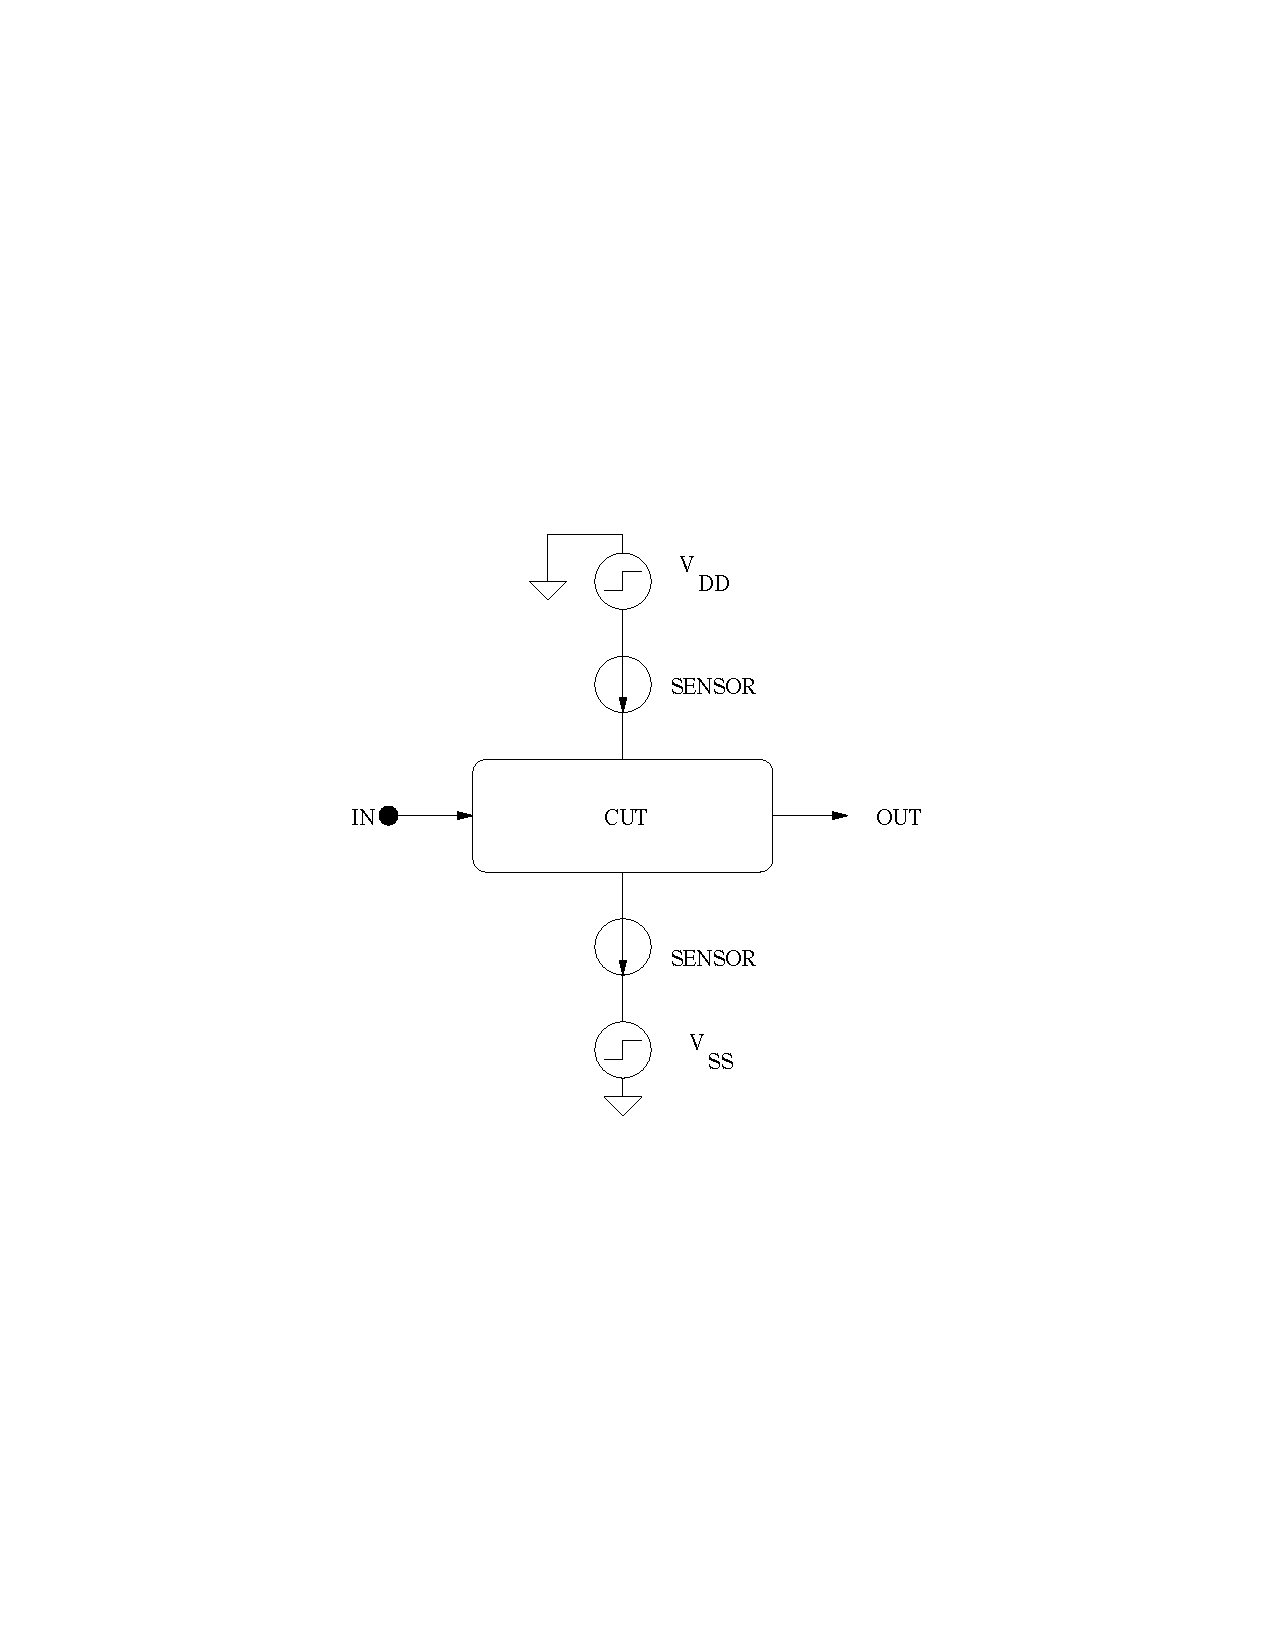
\includegraphics[width=0.5\linewidth]{cut}
  \end{figure}

\clearpage

%------------------------------------------------

\subsection{Ventajas de la técnica de $i_{DDQ}$}

\begin{itemize}
\item Monitoreo de corriente
\item Consumo de corriente mayor
\item Usado en estructuras CMOS estáticas
\end{itemize}
\newpage
Flujo de corriente:
\begin{figure}[h]
\centering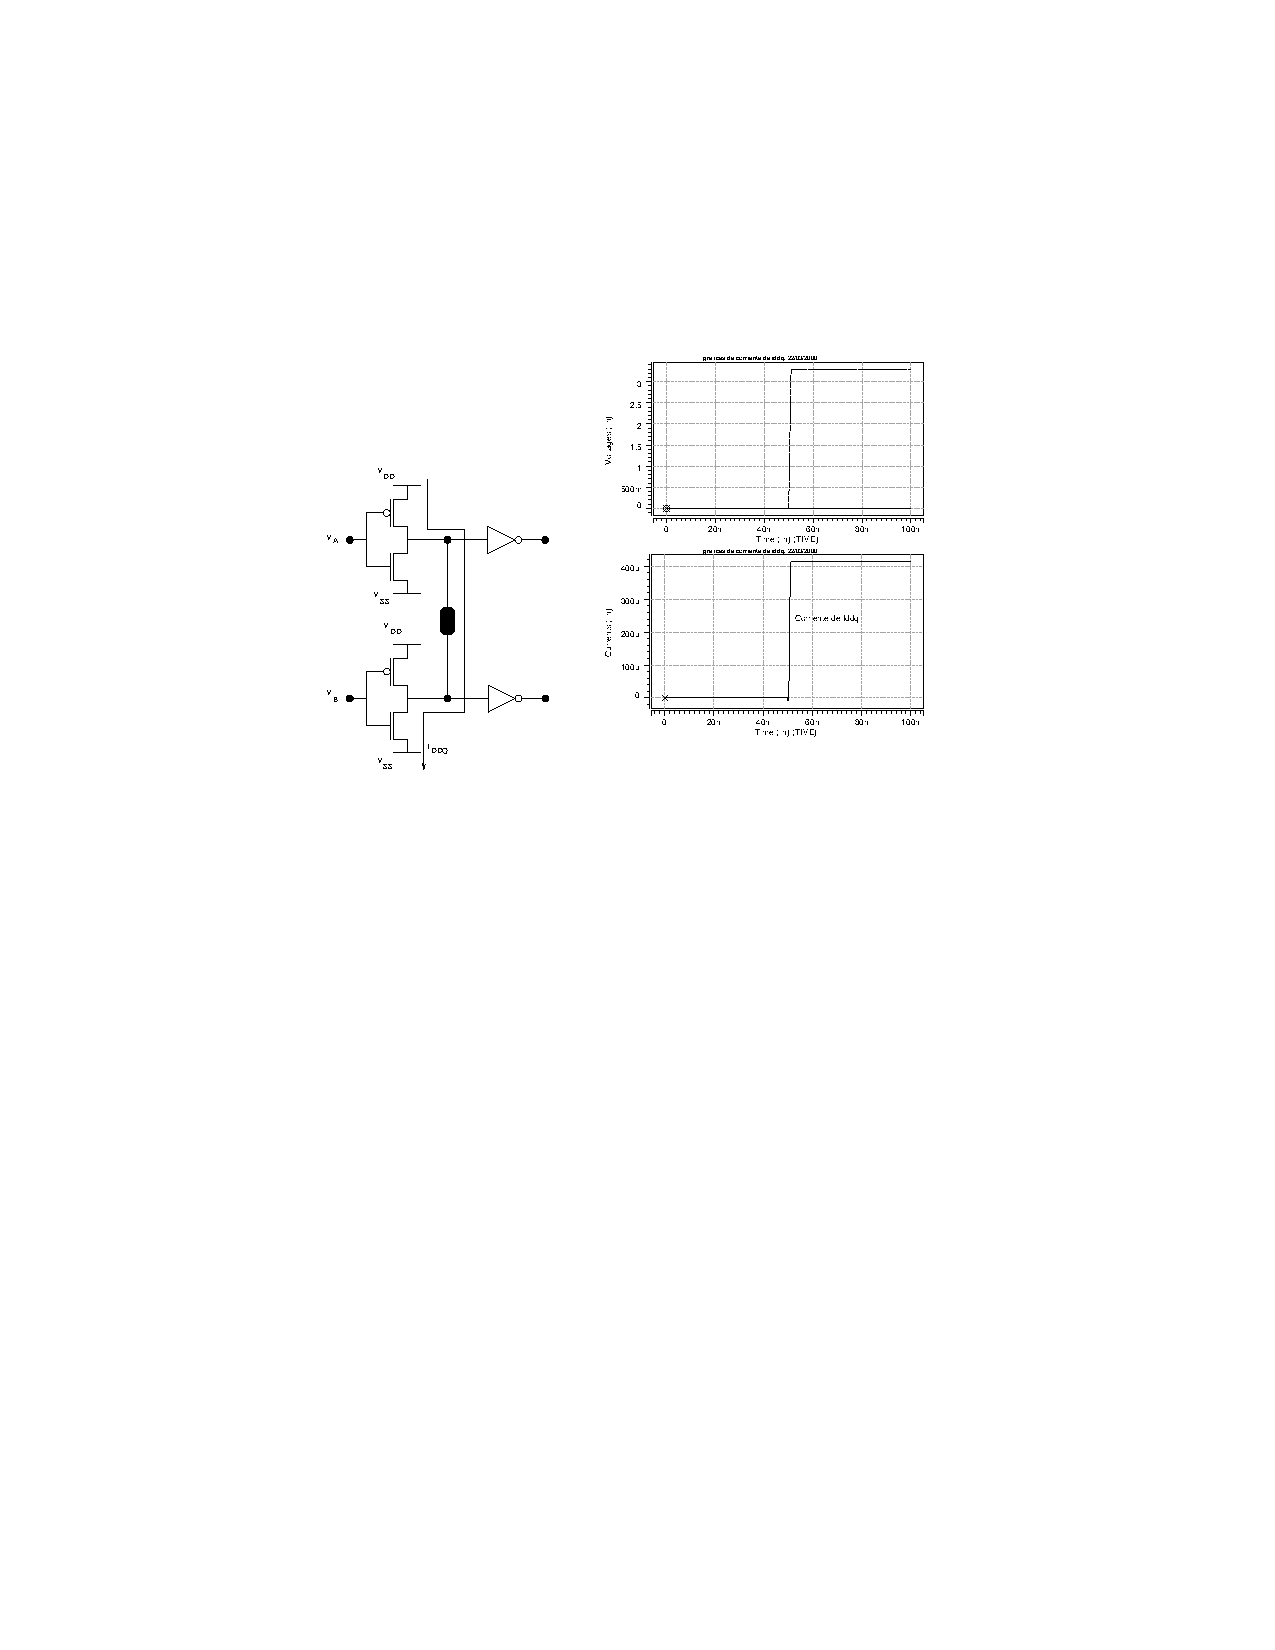
\includegraphics[width=0.6\linewidth]{iddq}
 % \caption{La prueba de $i_{DDQ}$}
\end{figure}

\clearpage

%------------------------------------------------

% \subsection{Corriente resultante de la prueba $i_{DDQ}$}

% \begin{figure}[h]
% \centering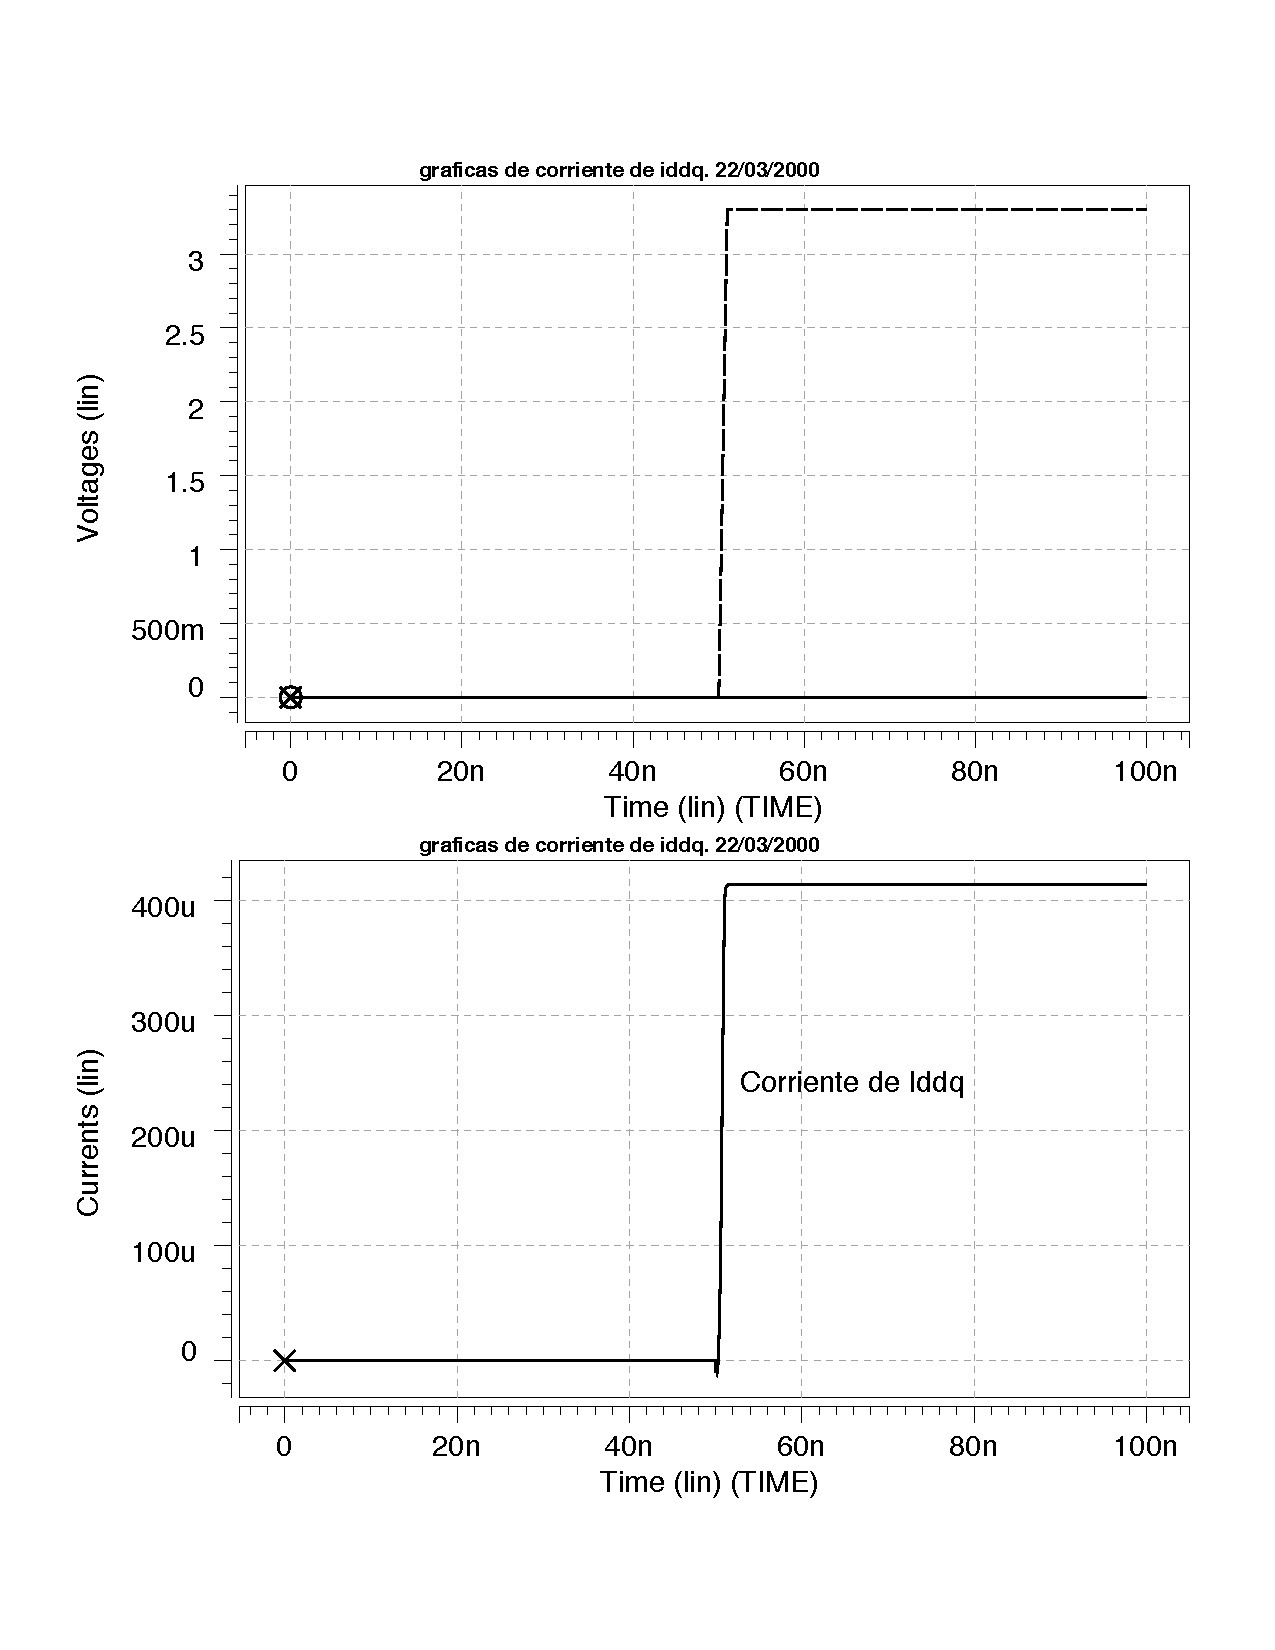
\includegraphics[width=0.33\linewidth]{g_iddq}
% % \caption{Corriente resultante de la prueba de $i_{DDQ}$}
% \end{figure}

% \clearpage

%------------------------------------------------

\subsection{Un único vector de prueba}

% \begin{table}[ht]
{\centering
\begin{tabular}{cc}
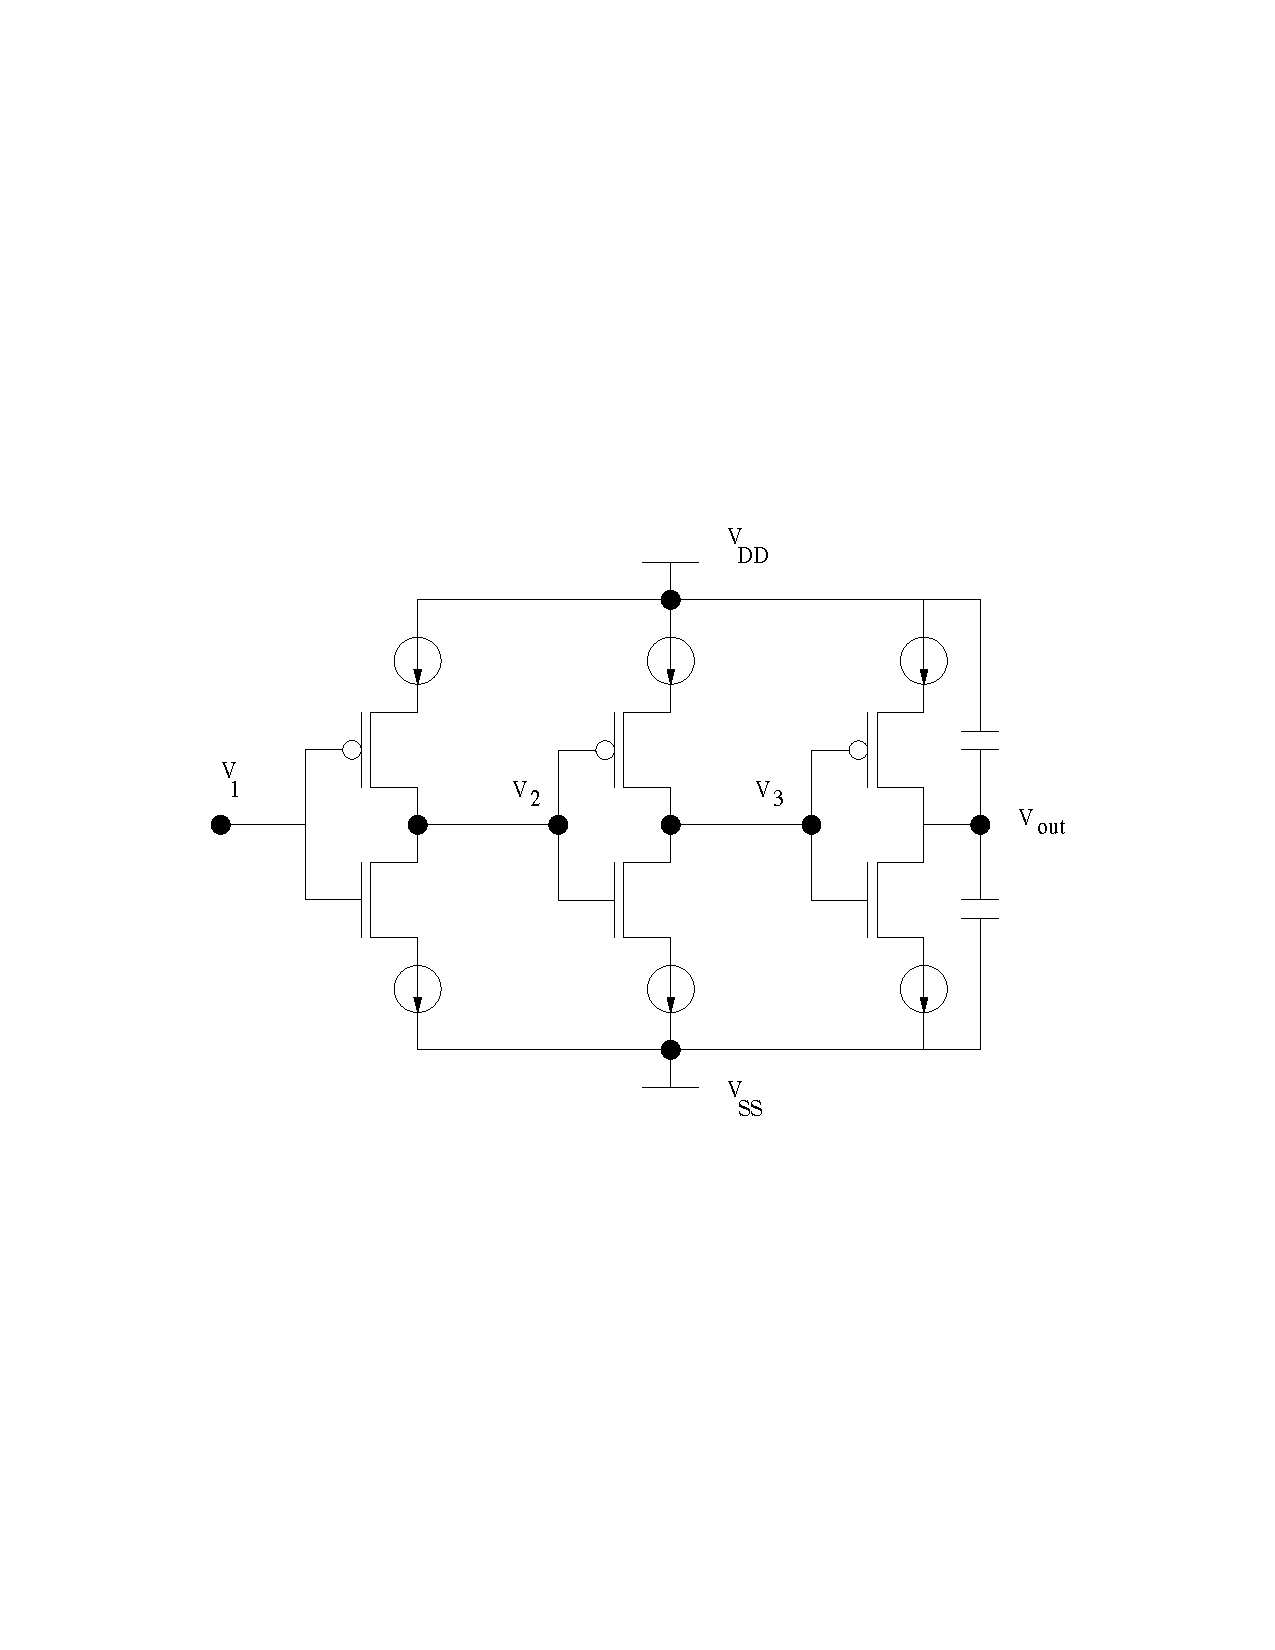
\includegraphics[width=0.4\linewidth]{buffer01}&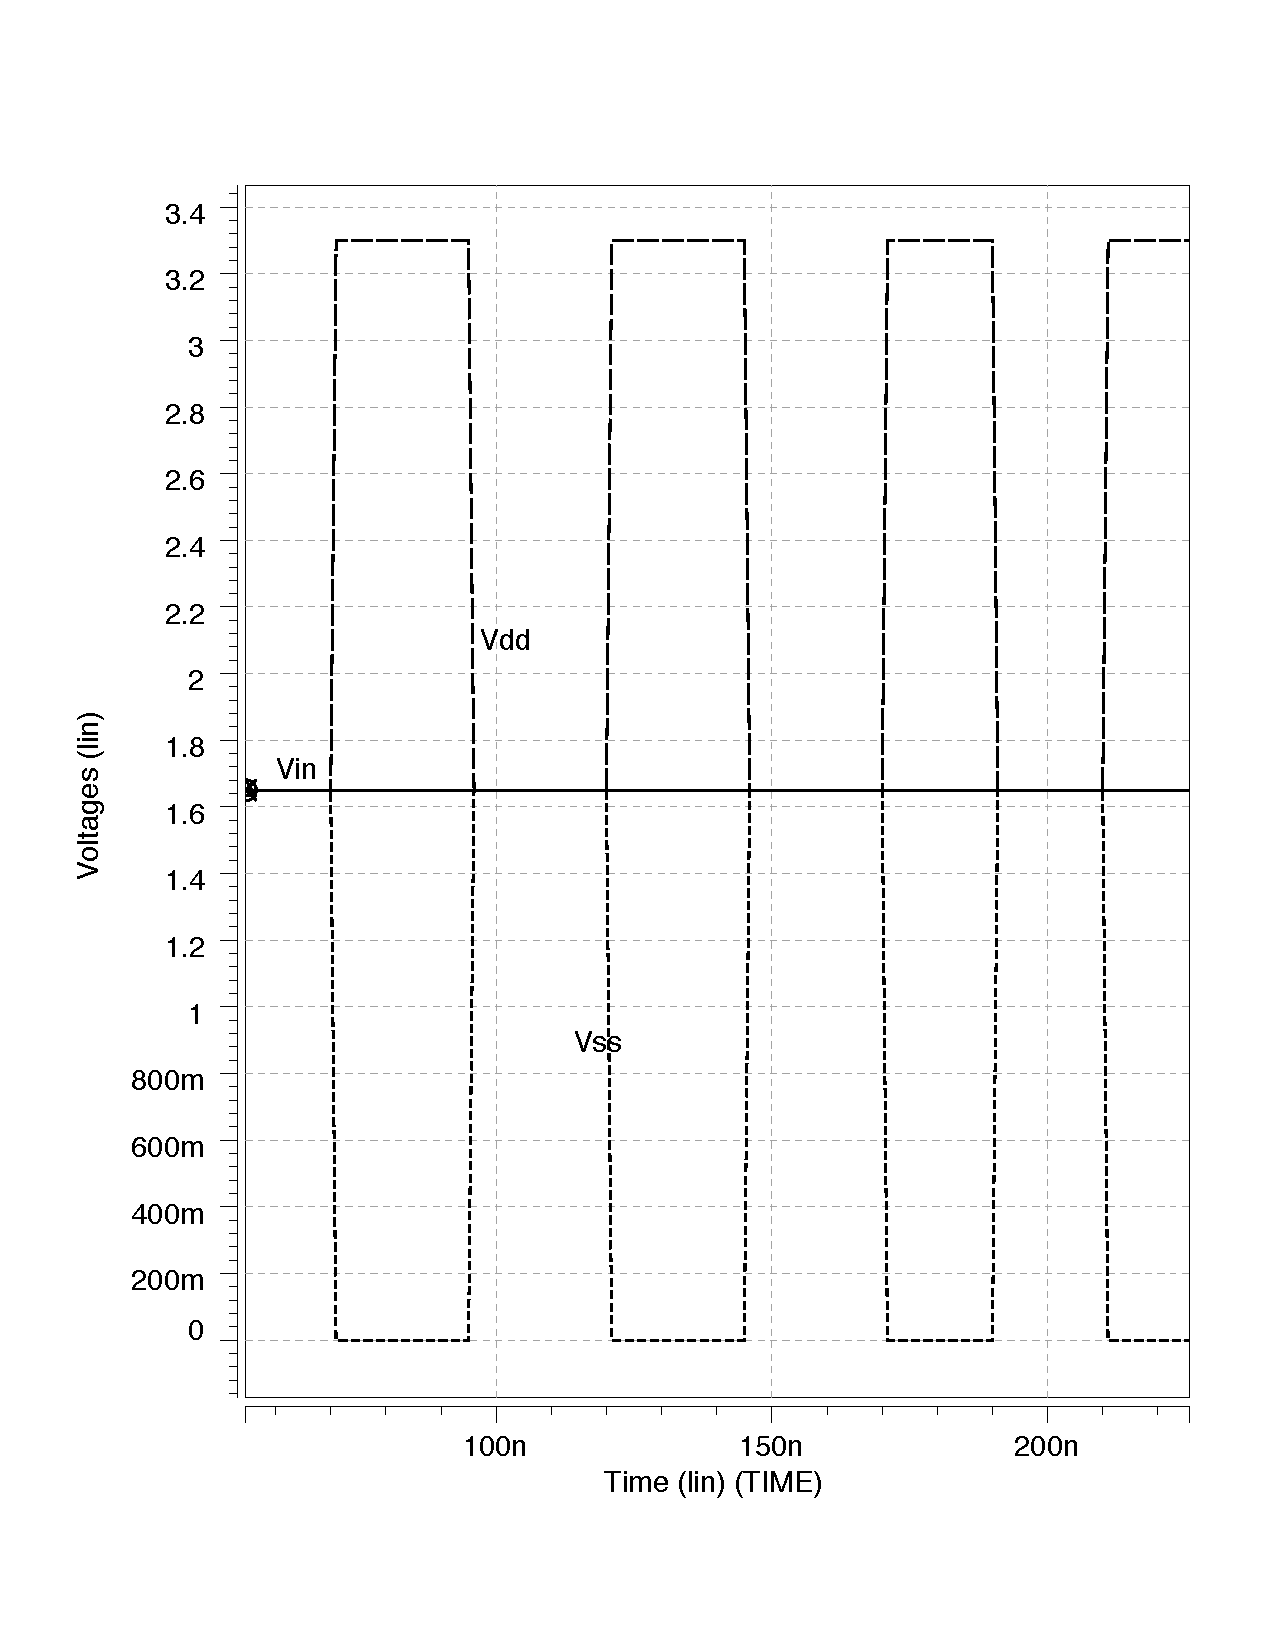
\includegraphics[width=0.4\linewidth]{iddqprt}\\
% \includegraphics[scale=1]{graphic3}&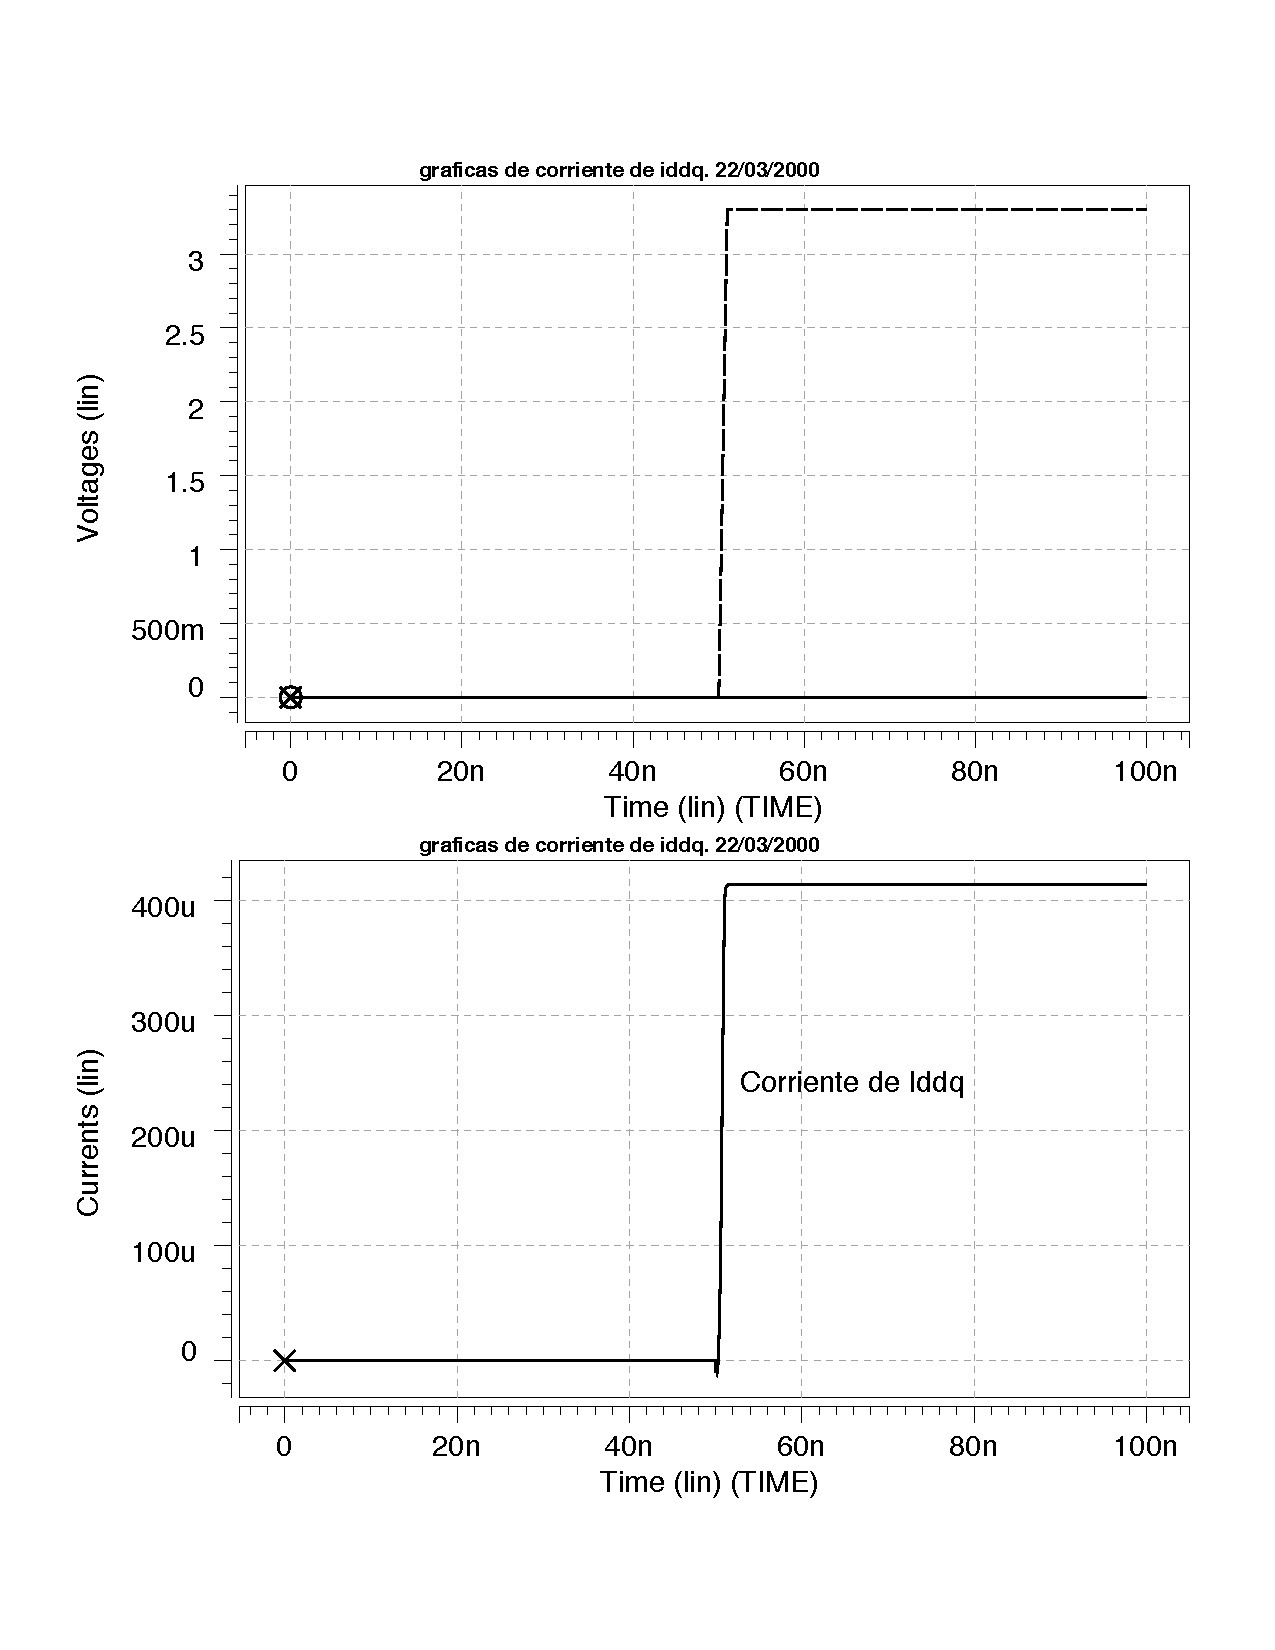
\includegraphics[scale=1]{g_iddq}\\
\end{tabular}}
% \label{tab:gt}
% \end{table}

% The most common definition of \mygreen{Murphy's Law} is as follows.

% \mybox{0.8\textwidth}{ % Example of encapsulating text in a colored box
% \begin{theorem}[Murphy (1949)]
% Anything that can go wrong, will go wrong.
% \end{theorem}
% }

% \begin{proof}
% A special case of this theorem is proven in the textbook.
% \end{proof}

% \begin{remark}
% This is a remark.
% \end{remark}

% \begin{algorithm}
% This is an algorithm.
% \end{algorithm}

\clearpage

%------------------------------------------------

\subsection{Modelo de primer orden}
\label{sec:model}

\begin{equation}
I_{DS}=\mu
C_{ox}\frac{W}{L}(V_{GS}-V_t)V_{DS}-\frac{1}{2}V_{DS}^2 \label{ec:lineal}
\end{equation}

\noindent Así, para $V_{DS}$ pequeños,

\begin{equation}
R_{transistor} \cong \frac{1}{\mu
  C_{ox}\frac{W}{L}(V_{GS}-V_t)} \label{ec:resistencia}
\end{equation}

\noindent la cual es la resistencia del transistor en funci\'on de
$V_{GS}$. De tal forma que podemos derivar:

\begin{equation}
V_o=V_{DD}\frac{R_n}{R_n+R_p}+V_{SS}\frac{R_p}{R_n+R_p} \label{ec:vout}
\end{equation}

\clearpage

\subsection{Caso simétrico: Modelo vs. Simulación}
\label{sec:simetrico}

\begin{table}[ht]
% \caption{Modelo y simulación.}
\centering
\begin{tabular}{cc}
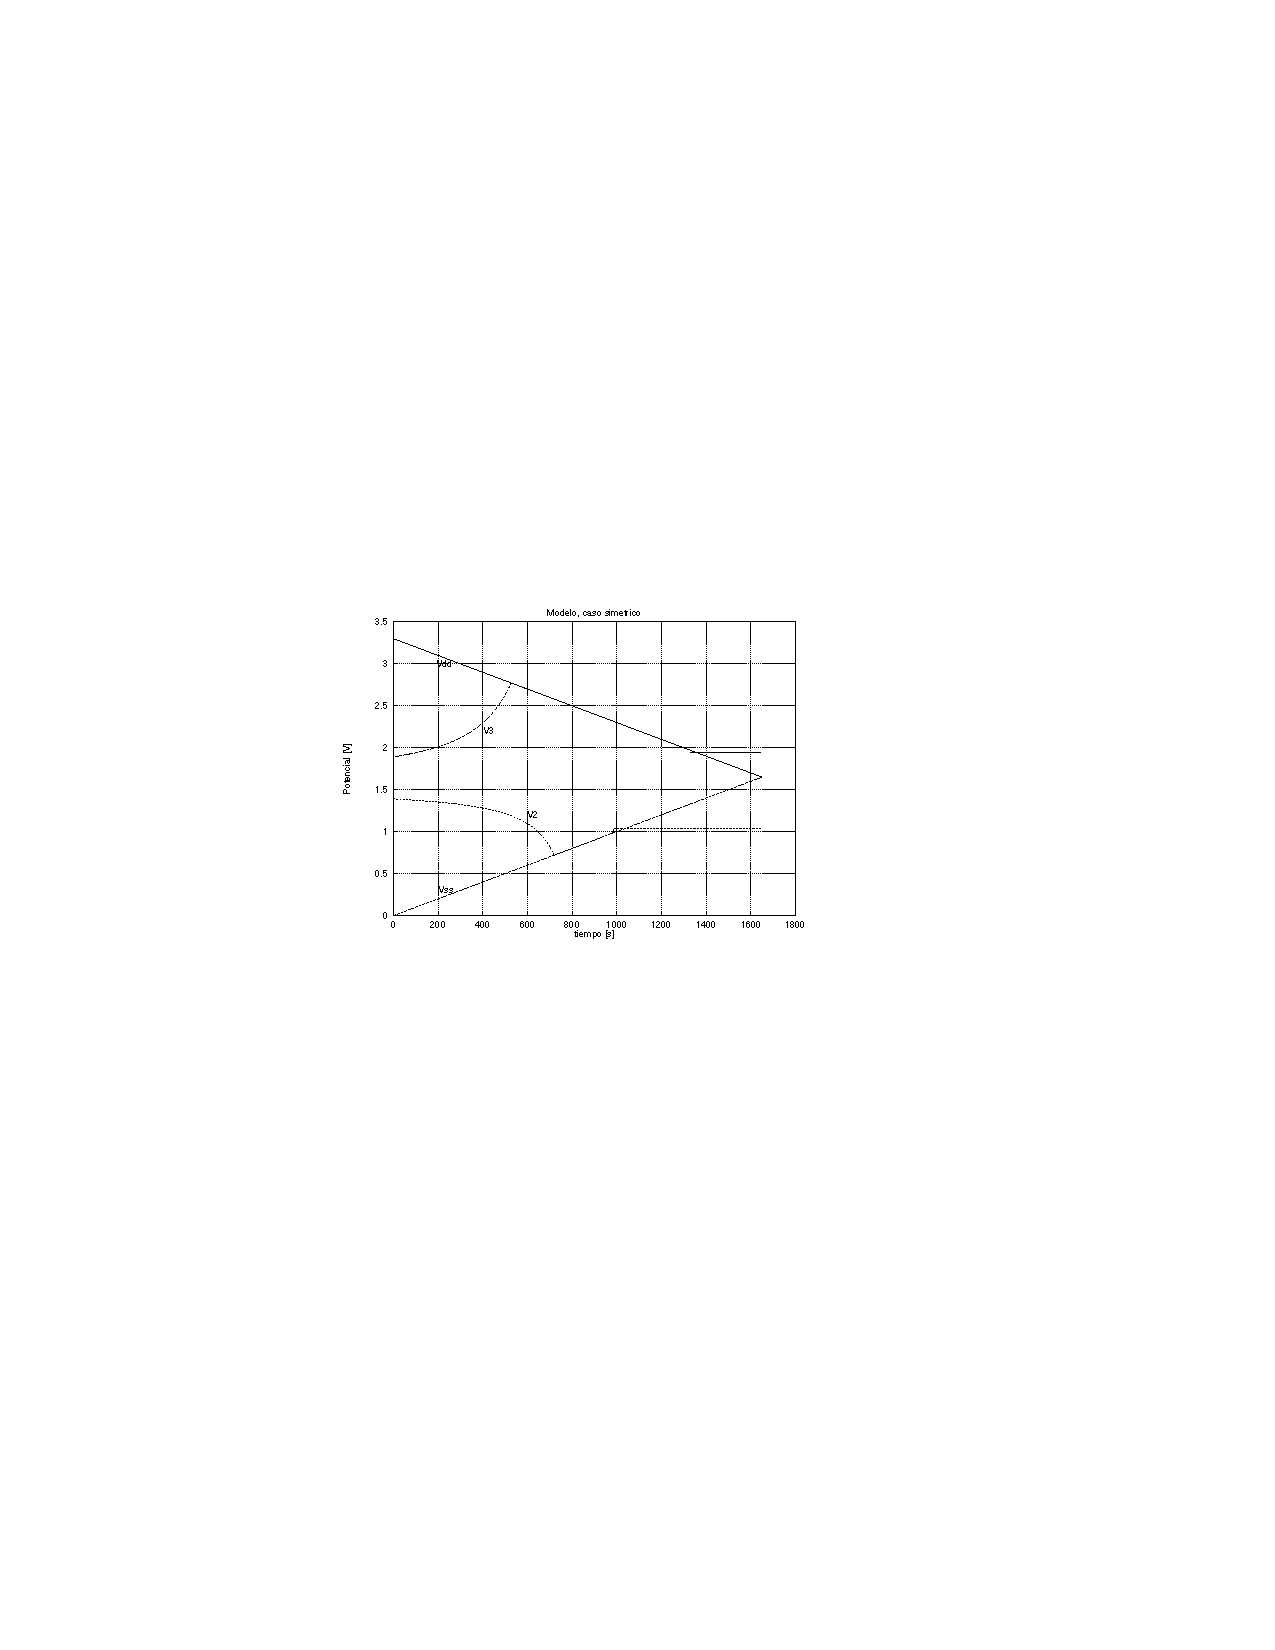
\includegraphics[width=0.45\linewidth]{modelSimetrico}&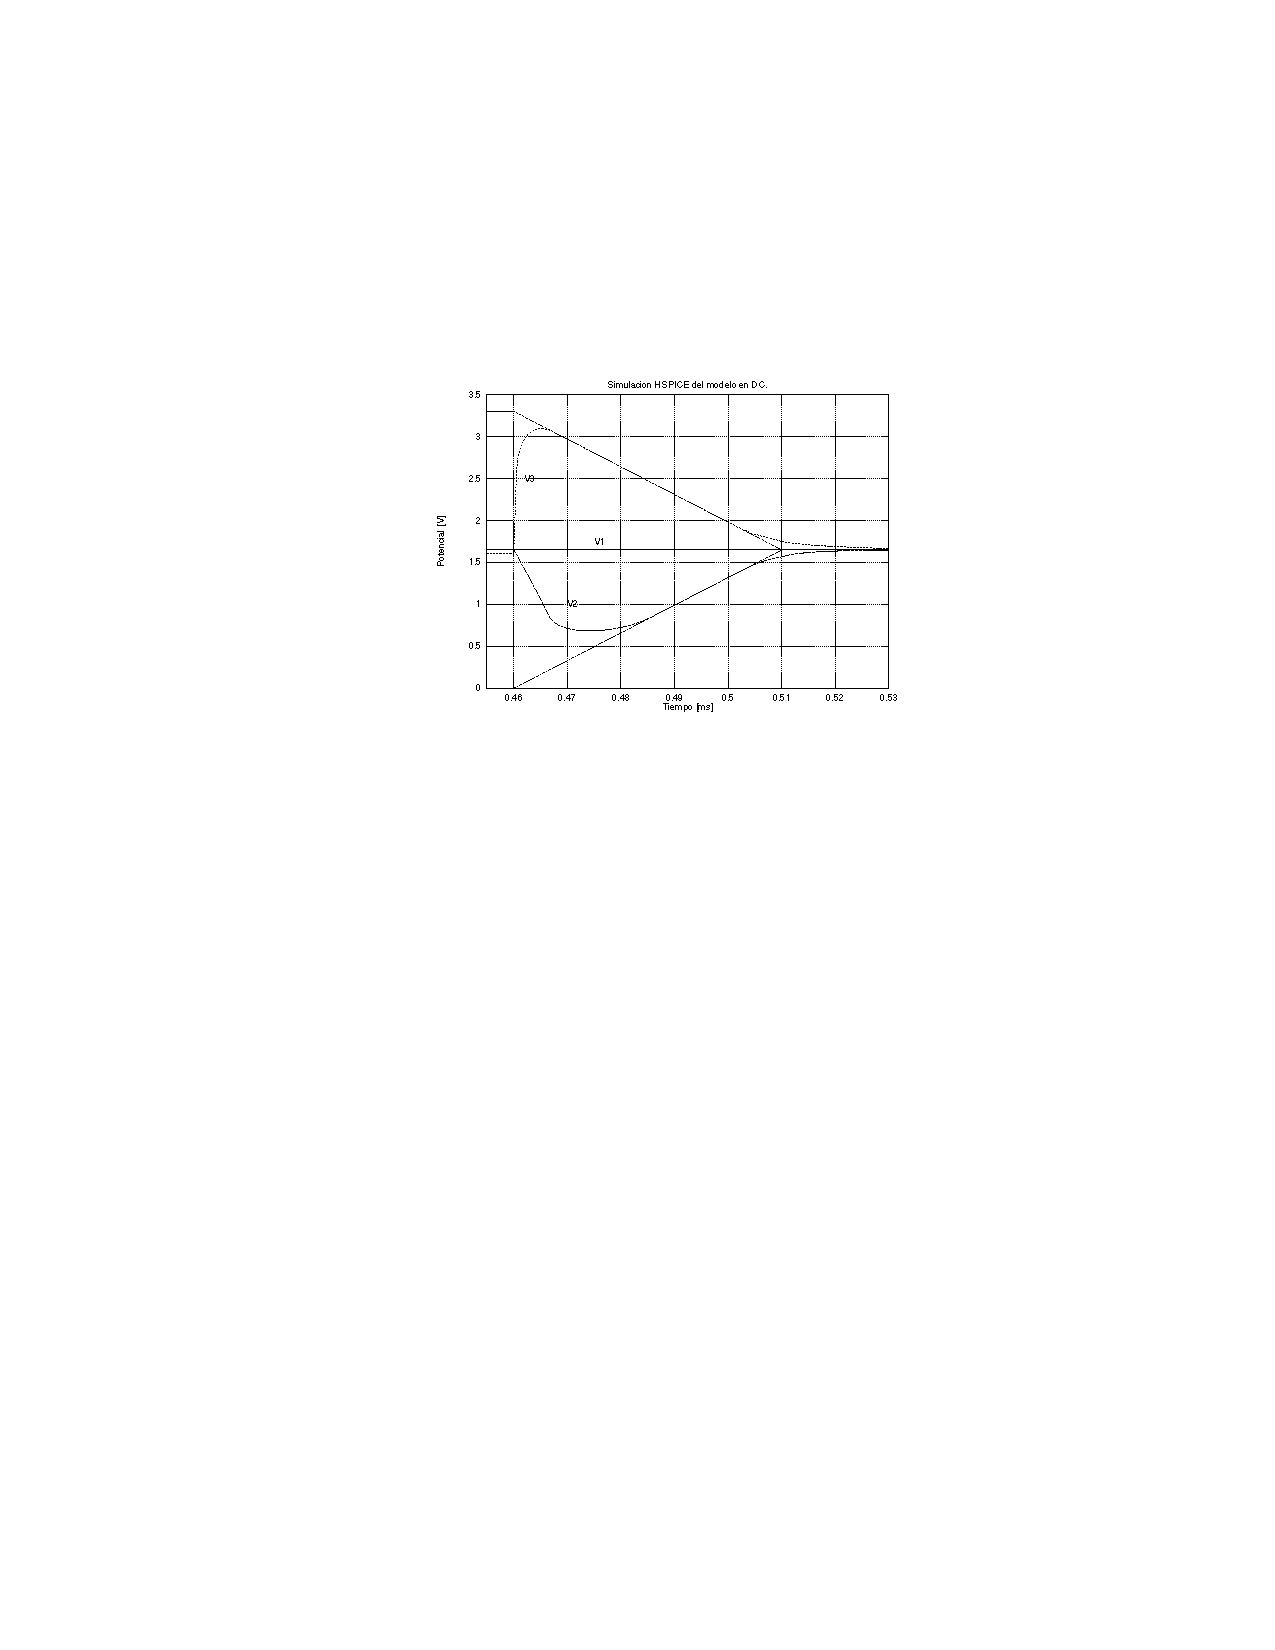
\includegraphics[width=0.45\linewidth]{SimSimetrico}\\

% \includegraphics[scale=1]{graphic3}&\includegraphics[scale=1]{graphic4}\\
\end{tabular}
\label{tab:simetrico}
\end{table}

\clearpage

\subsubsection{Potenciales: Modelo y simulación del caso asimétrico (a)}
\label{sec:asimetricoA}

\begin{table}[ht]
% \caption{Potenciales: Modelo y simulación del caso asimétrico (a)}
\centering
\begin{tabular}{cc}
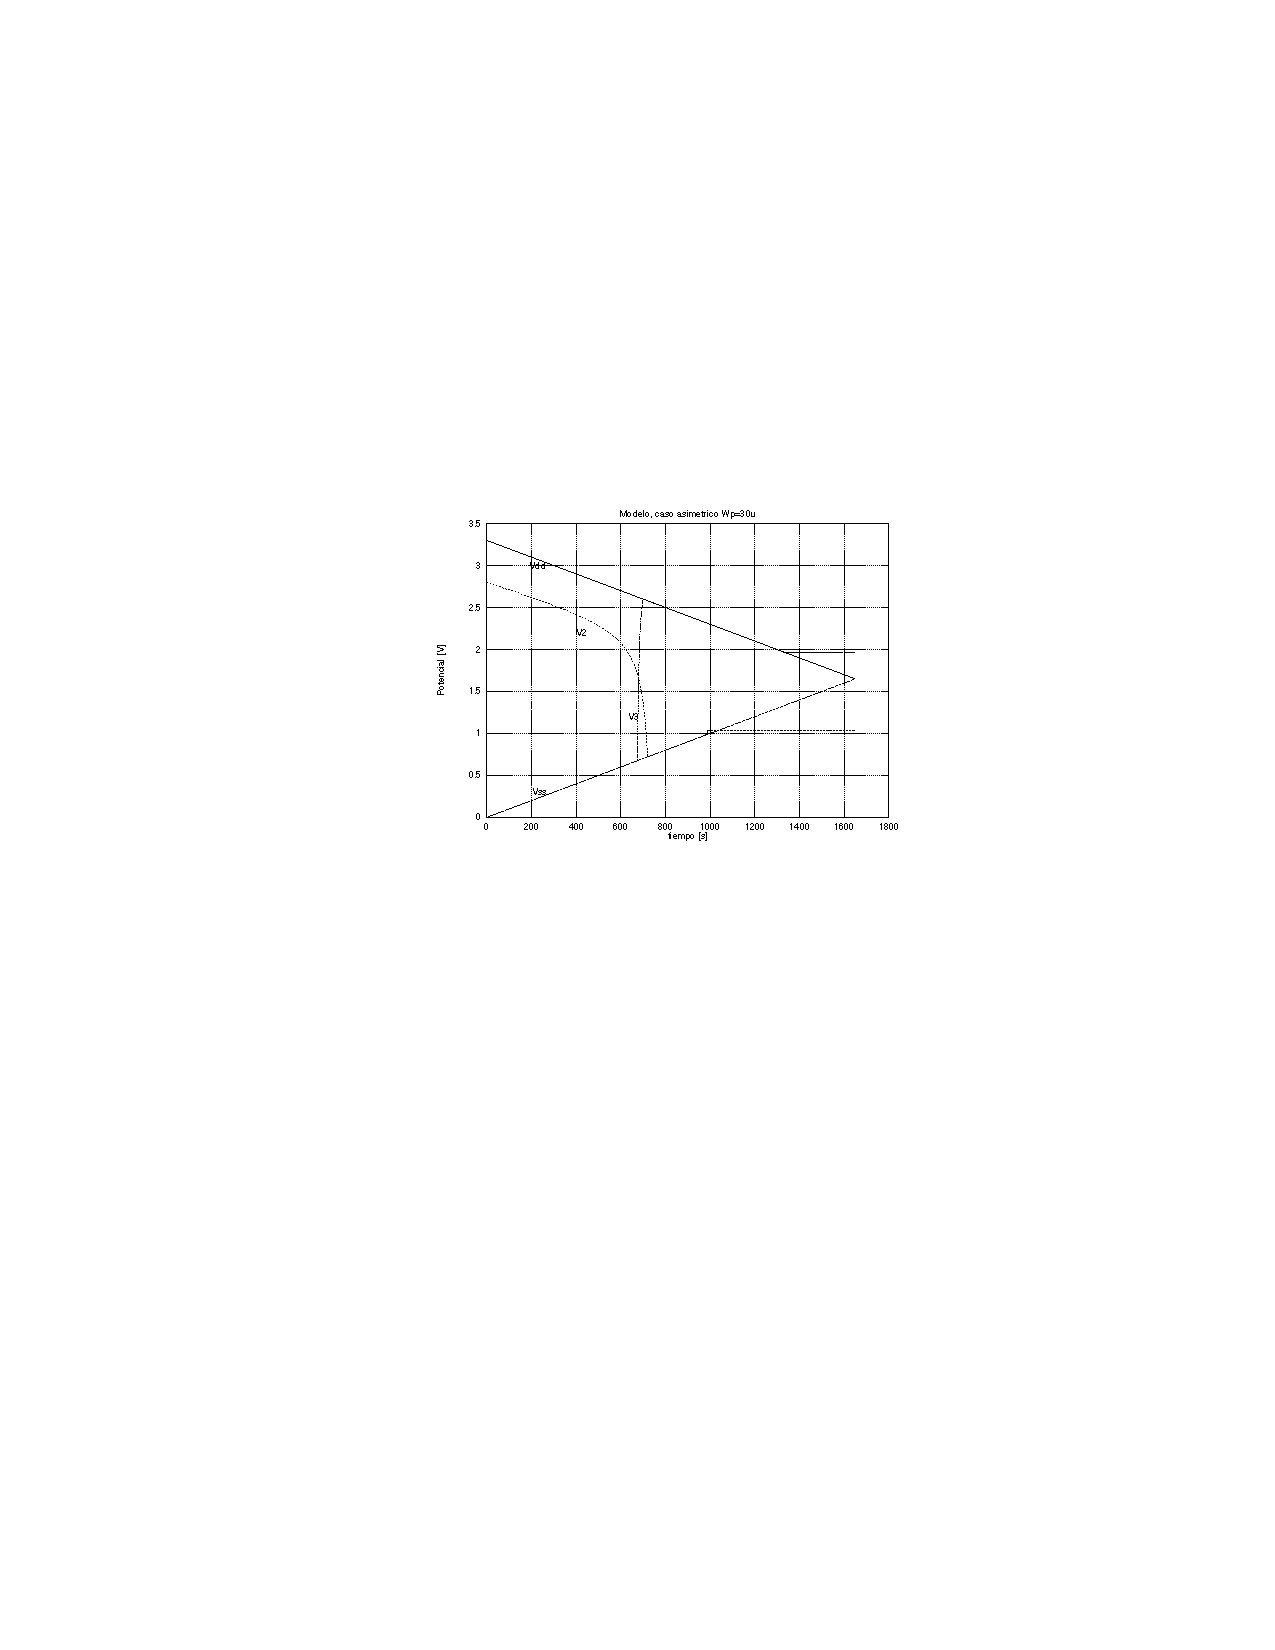
\includegraphics[width=0.45\linewidth]{ModeloAsimetricoA}&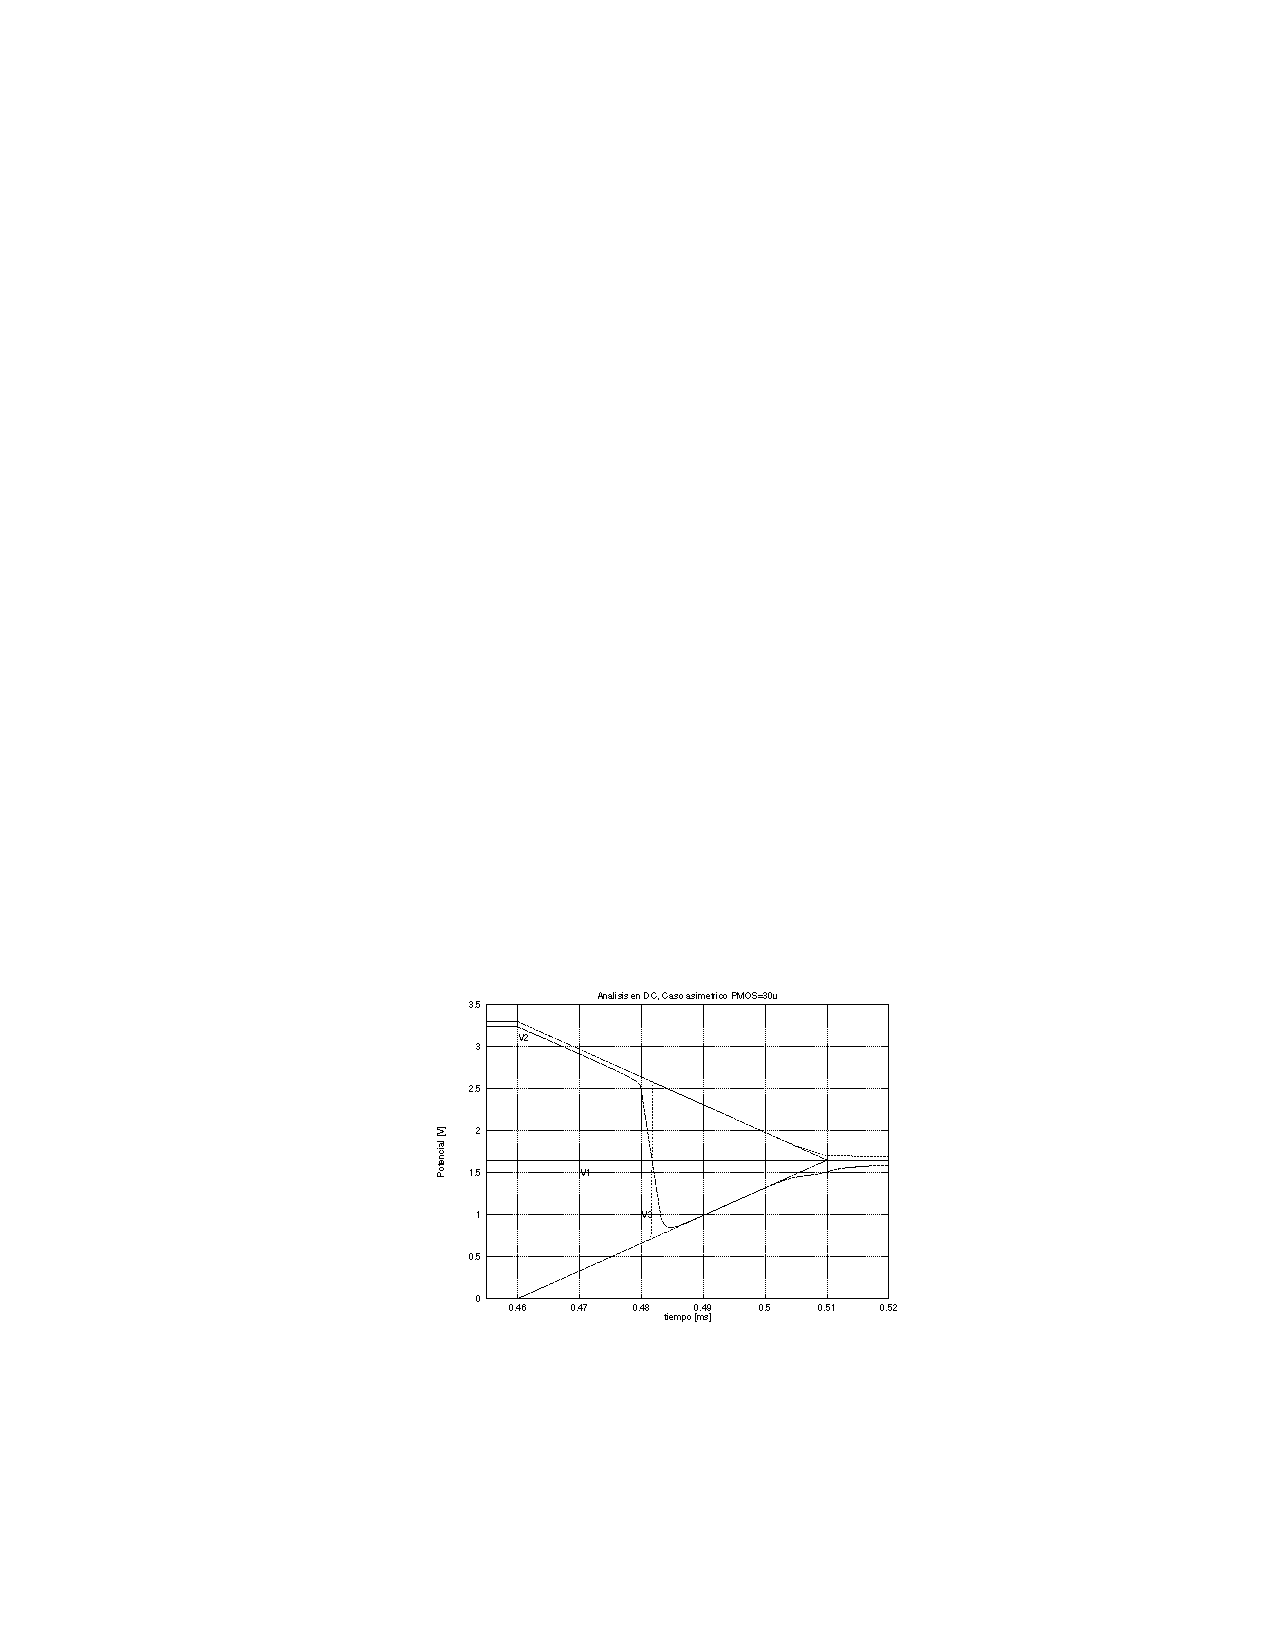
\includegraphics[width=0.45\linewidth]{SimulacionAsimetricoA}\\
\end{tabular}
\label{tab:gt}
\end{table}

\clearpage

\subsubsection{Potenciales: Modelo y simulación del caso asimétrico (b)}
\label{sec:asimetricoB}

\begin{table}[ht]
% \caption{Potenciales: Modelo y simulación del caso asimétrico (a)}
\centering
\begin{tabular}{cc}
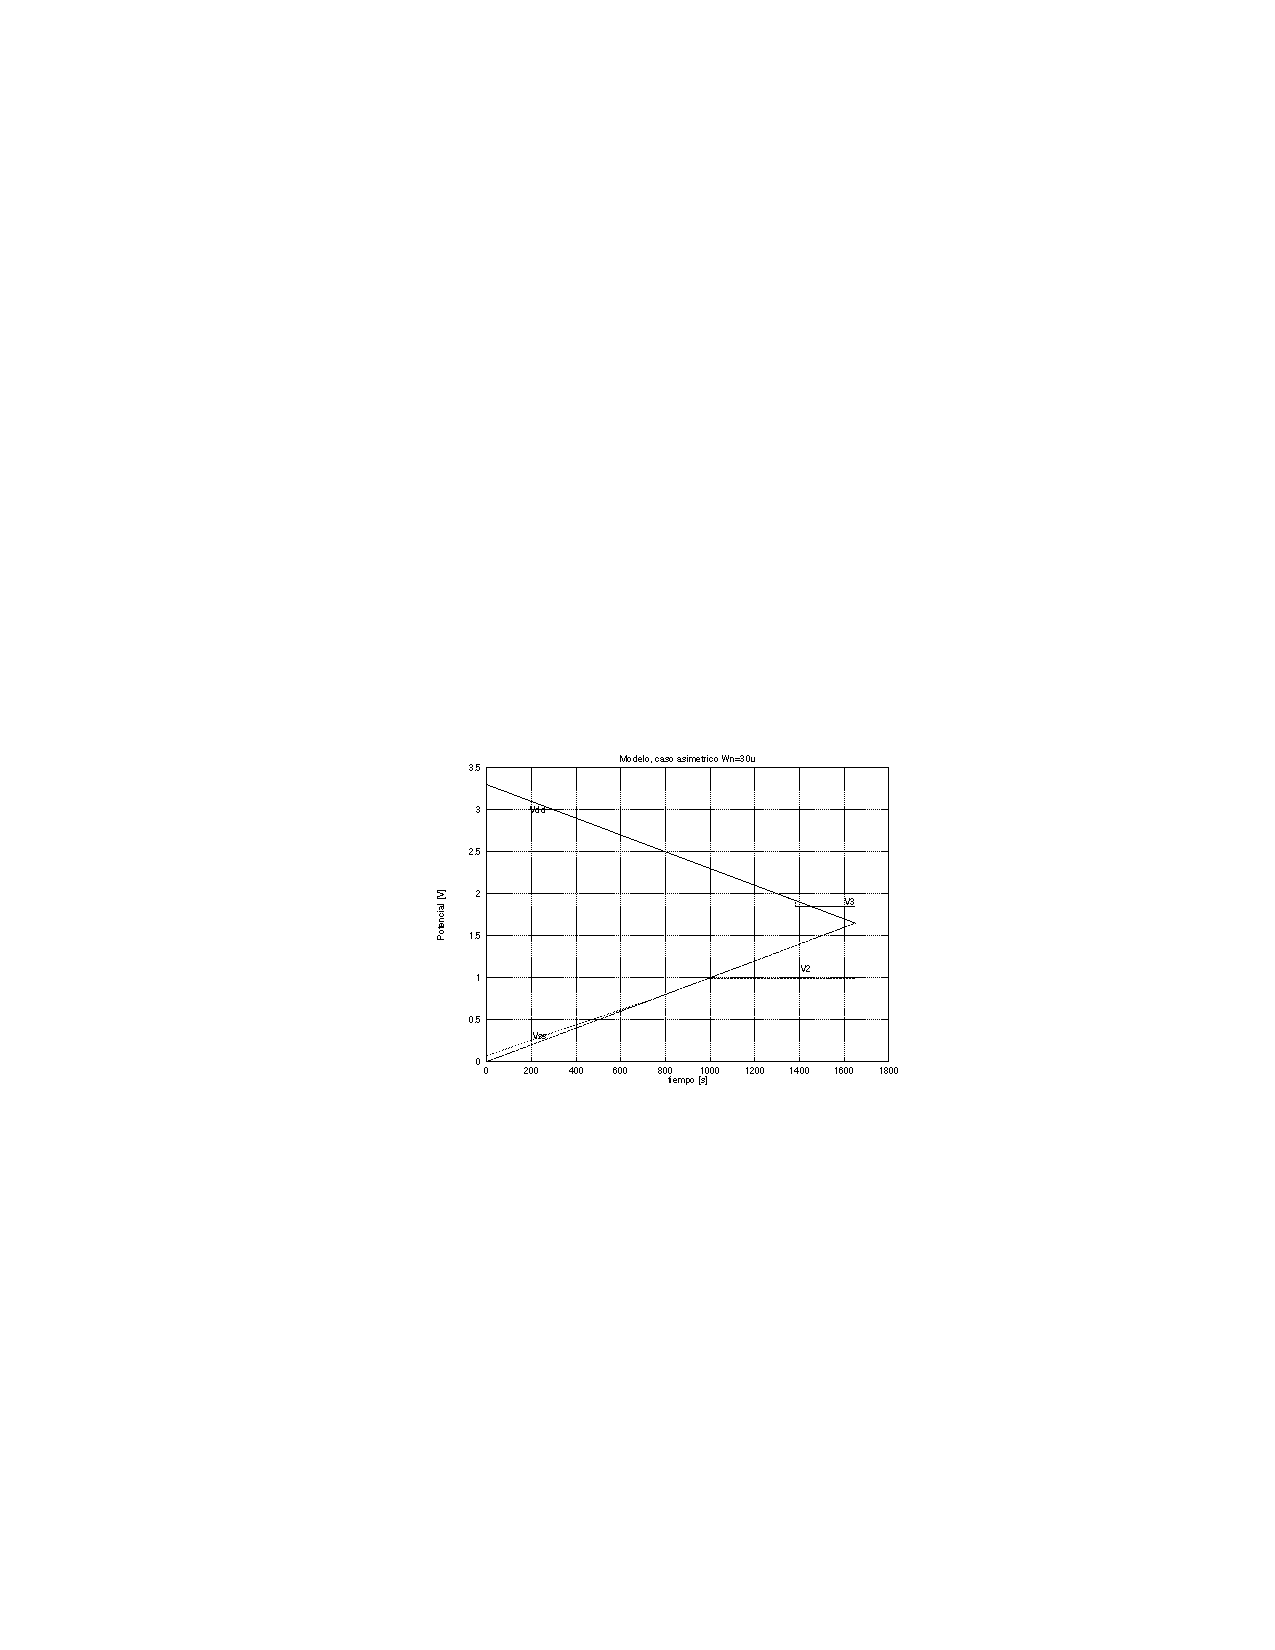
\includegraphics[width=0.45\linewidth]{ModeloAsimetricoB}&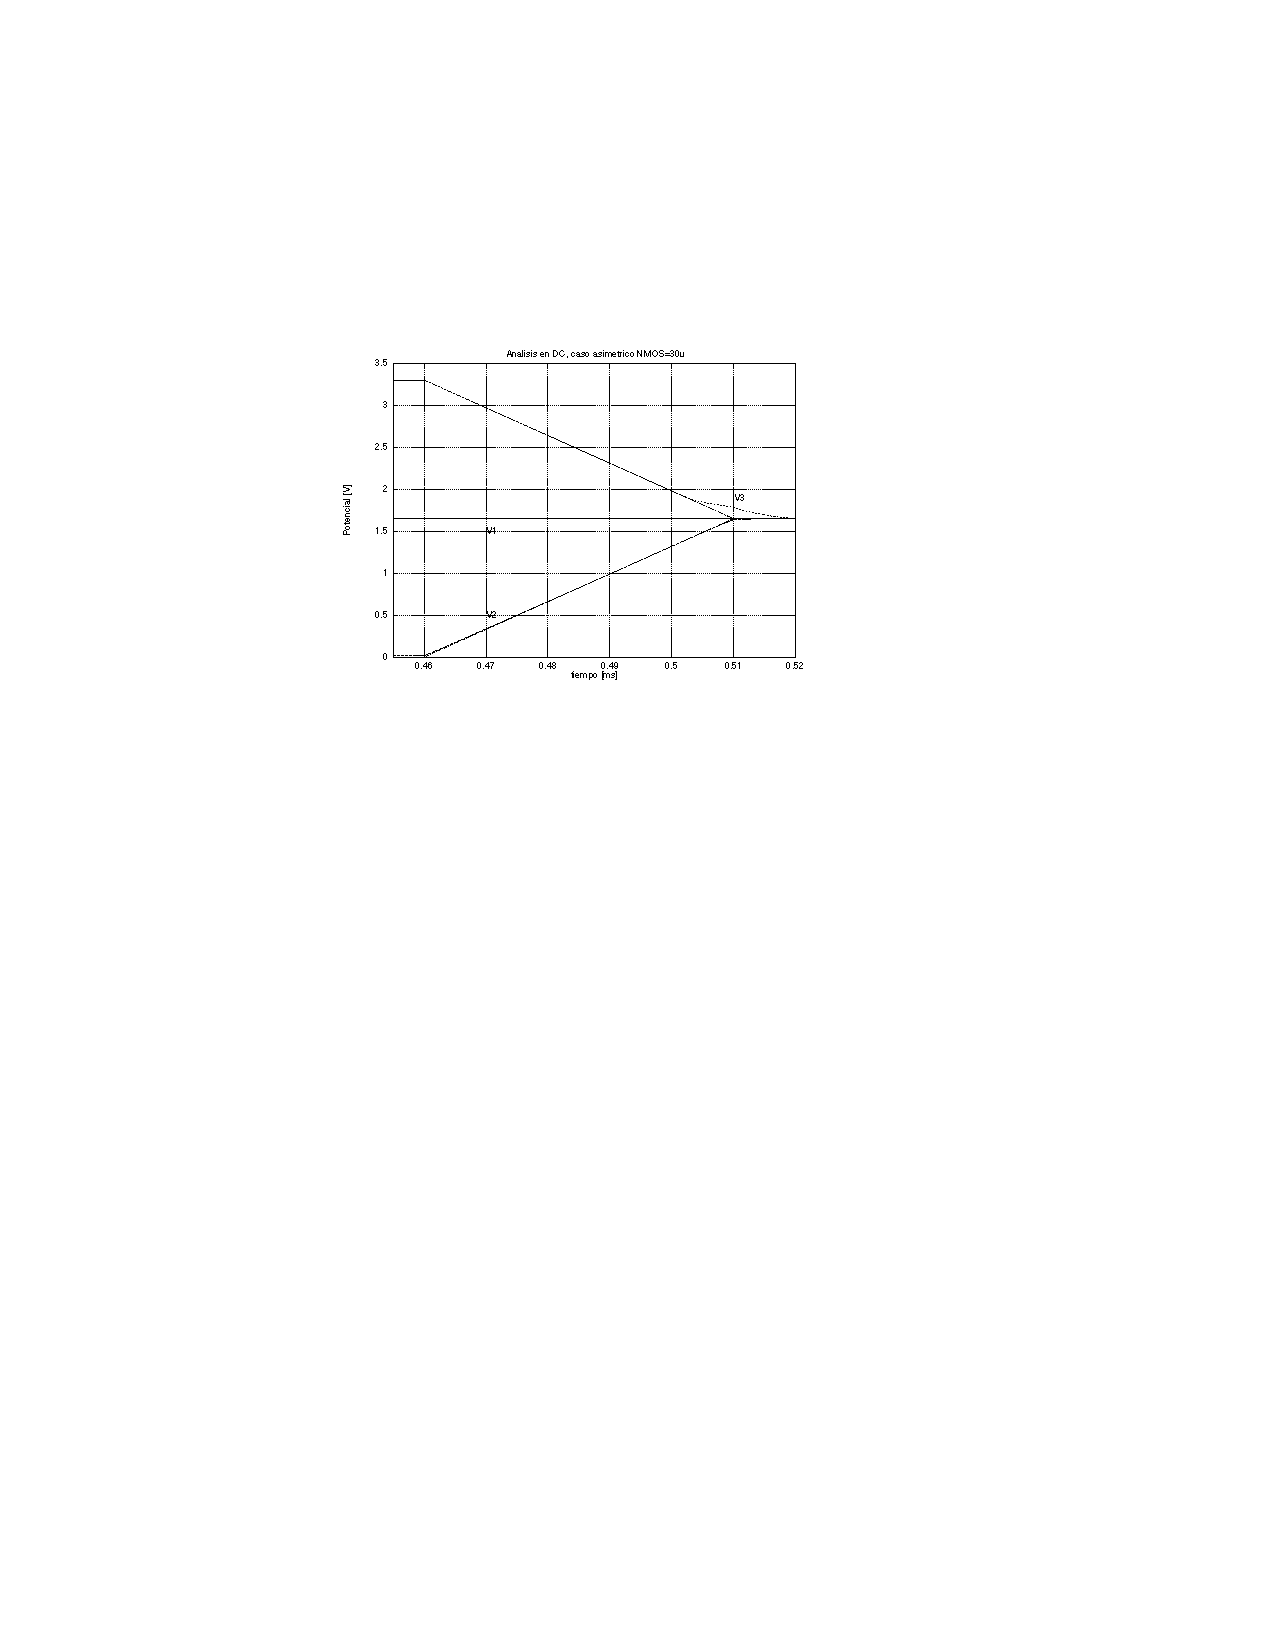
\includegraphics[width=0.45\linewidth]{SimulacionAsimetricoB}\\
\end{tabular}
\label{tab:gt}
\end{table}

\clearpage

\subsubsection{Análisis de Corriente (a) Cuasi-simétrico (b) Asimétrico}
\label{sec:iddAnalysis}

\begin{table}[ht]
% \caption{Potenciales: Modelo y simulación del caso asimétrico (a)}
\centering
\begin{tabular}{cc}
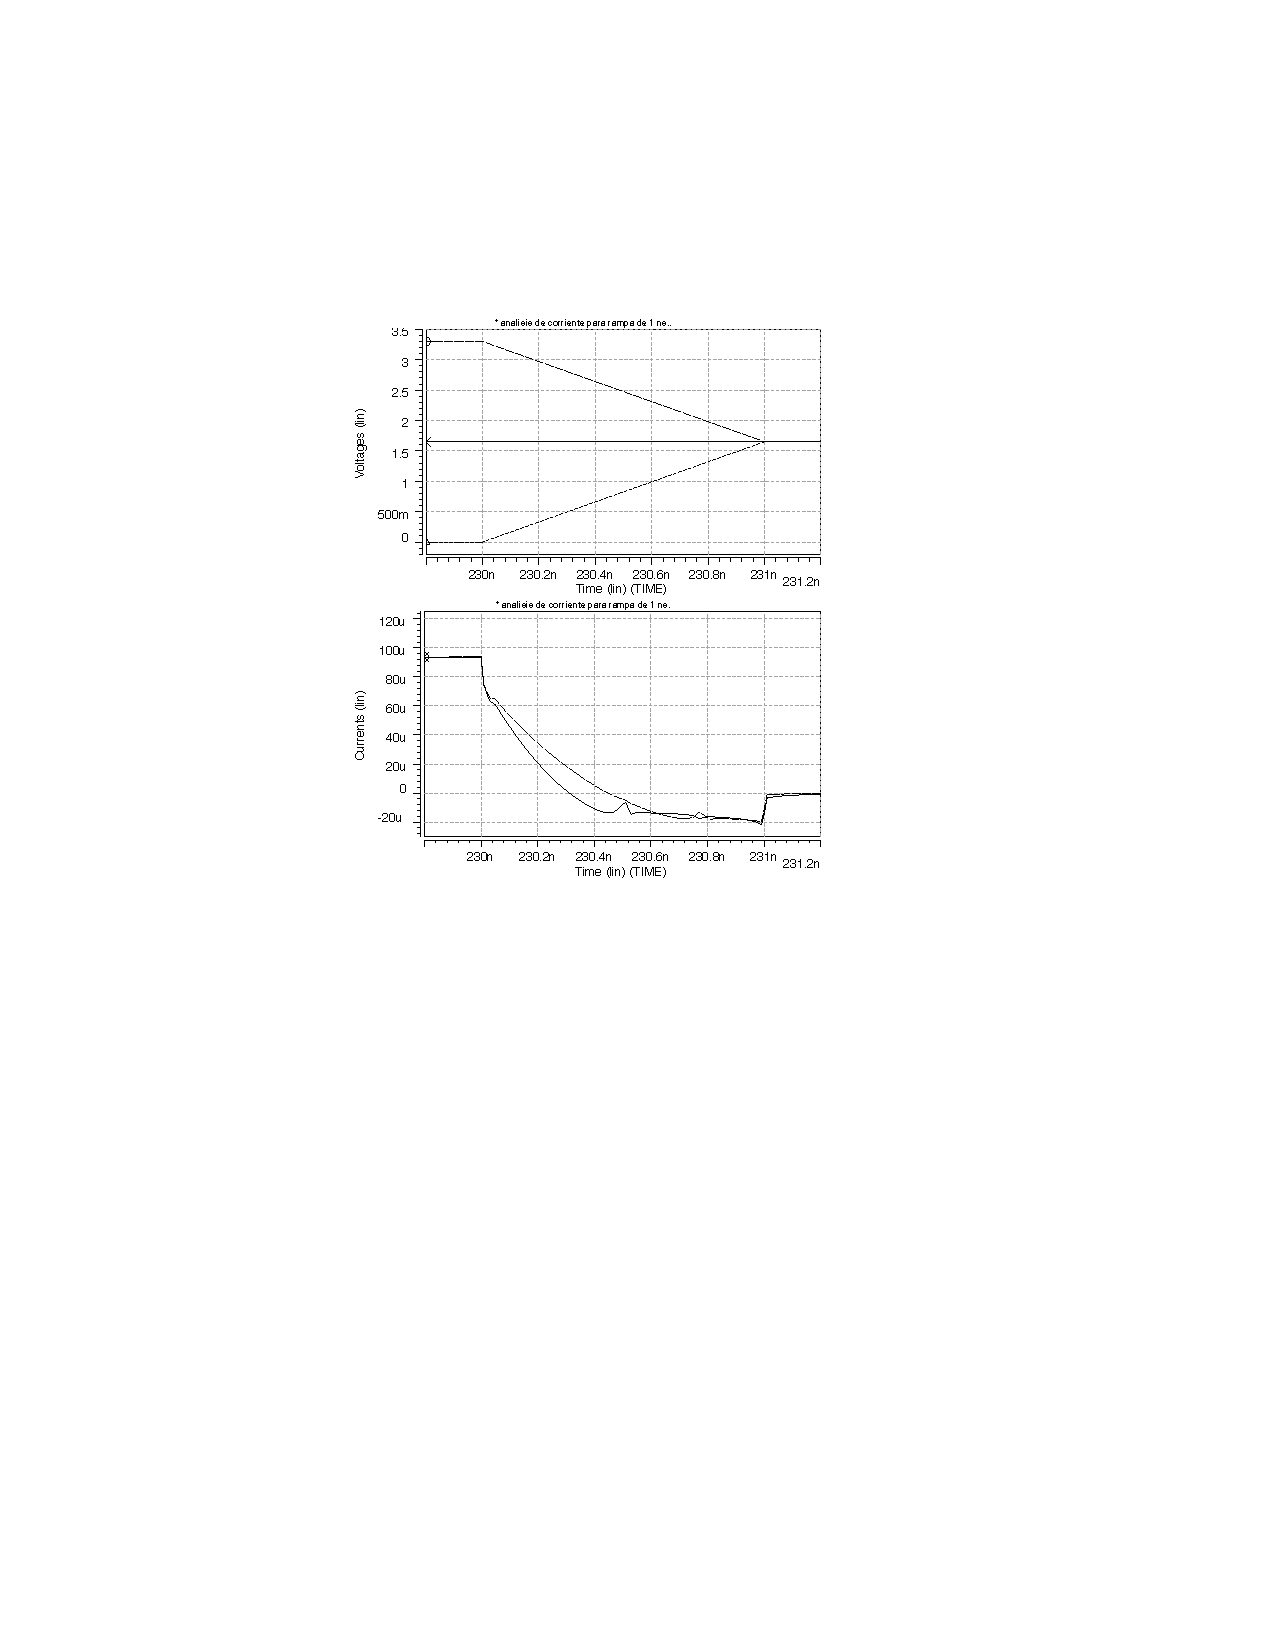
\includegraphics[width=0.35\linewidth]{iddAnalysisCuasiSimetrico}&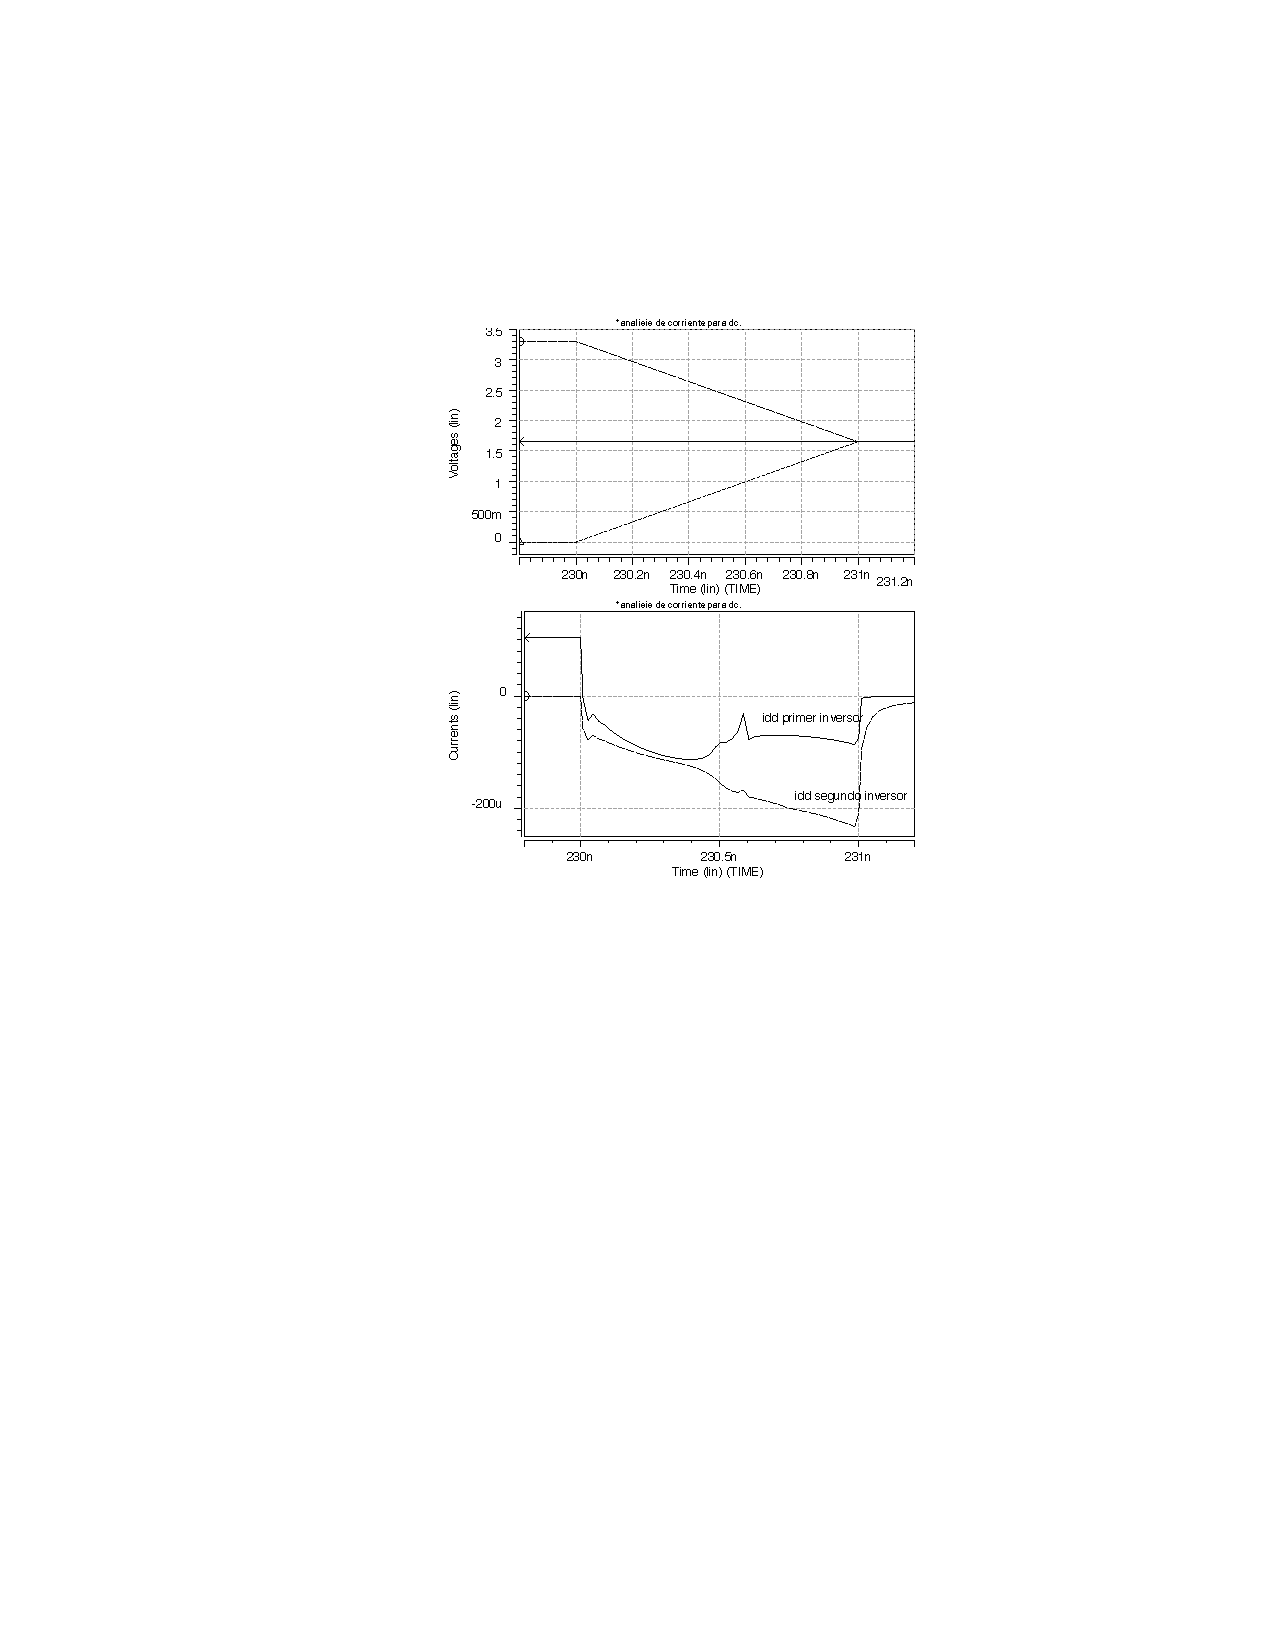
\includegraphics[width=0.35\linewidth]{iddAnalysisAsimetrico}\\
\end{tabular}
\label{tab:gt}
\end{table}

\clearpage

Tanto la zona estable como la rampa del vector de prueba presentan
flujo de corriente:

\begin{figure}[h]
  \centering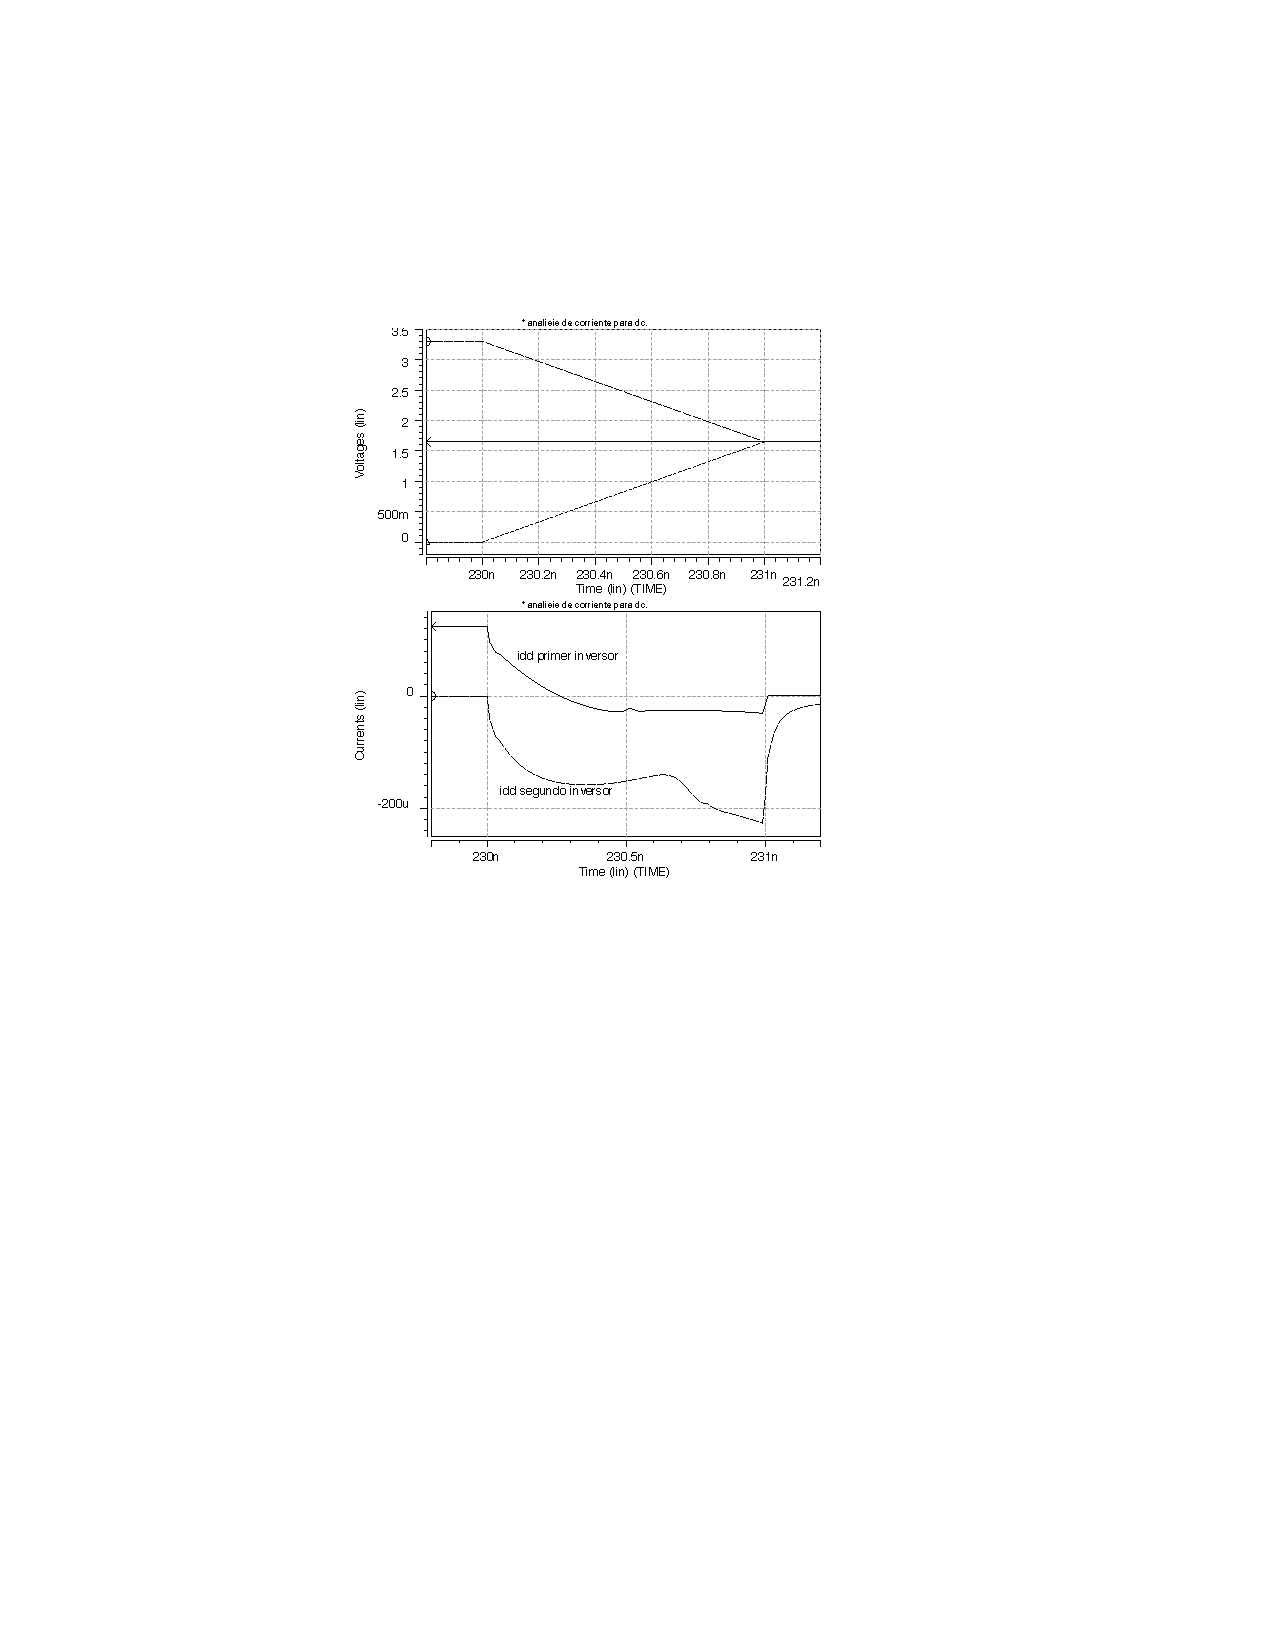
\includegraphics[width=0.35\linewidth]{iddAnalysisAsimetrico2}
\end{figure}

\clearpage

\subsection{$i_{DD}$ en un celda básica real}
\label{sec:adder}

\begin{figure}[h]
  \centering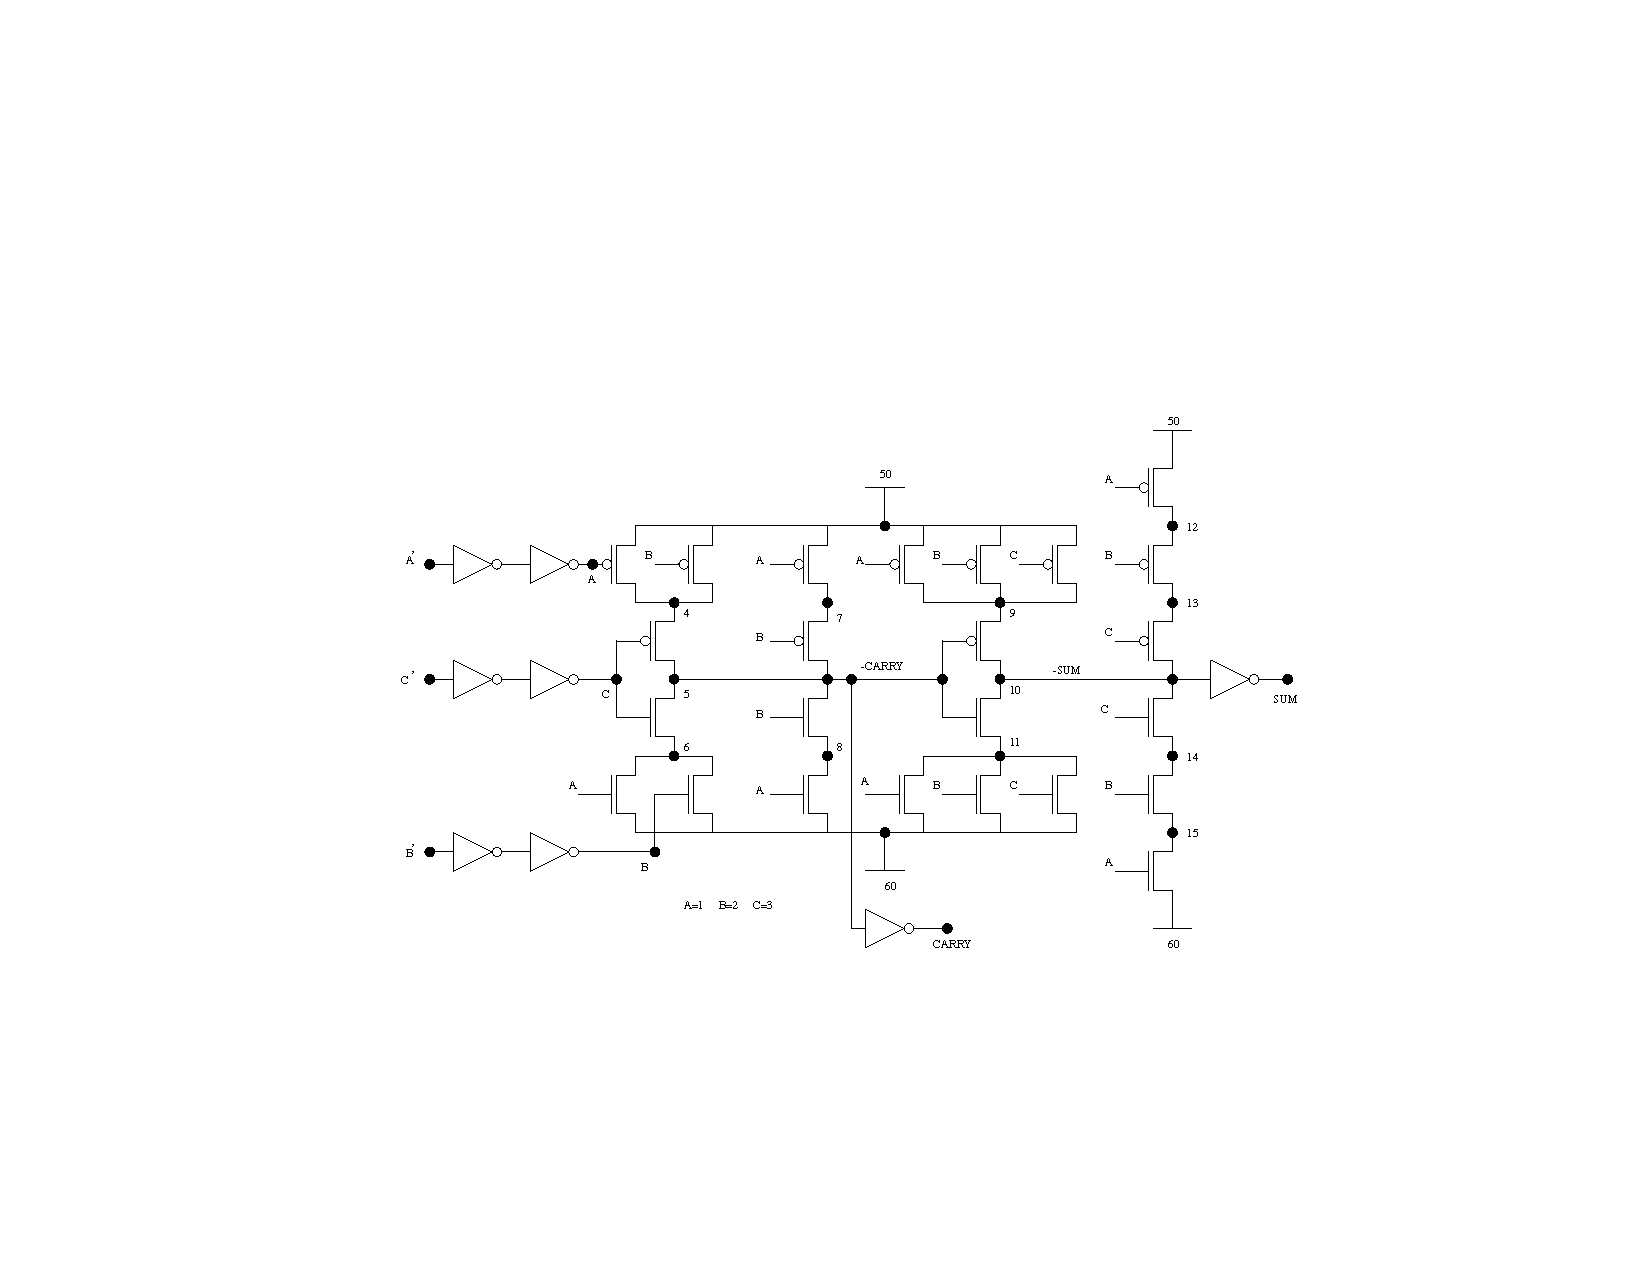
\includegraphics[width=0.65\linewidth]{fullAdder}
\end{figure}

\clearpage

Layout del Circuito Sumador completo optimizado:

\begin{figure}[h]
  \centering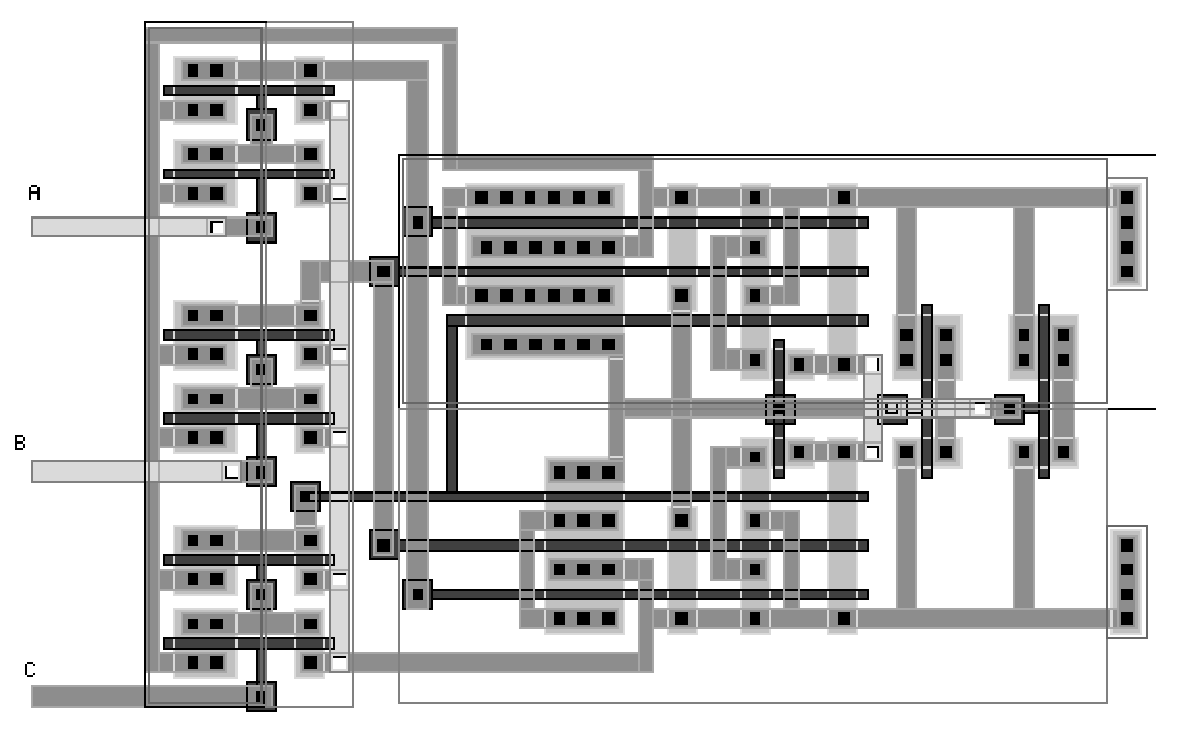
\includegraphics[width=0.65\linewidth]{adder8}
\end{figure}

\clearpage

Ejemplos de resultados:
% \subsubsection{Ejemplos de resultados}
% \label{sec:exFaultResult}

\begin{table}[ht]
  \centering
  \begin{tabular}{cc}
    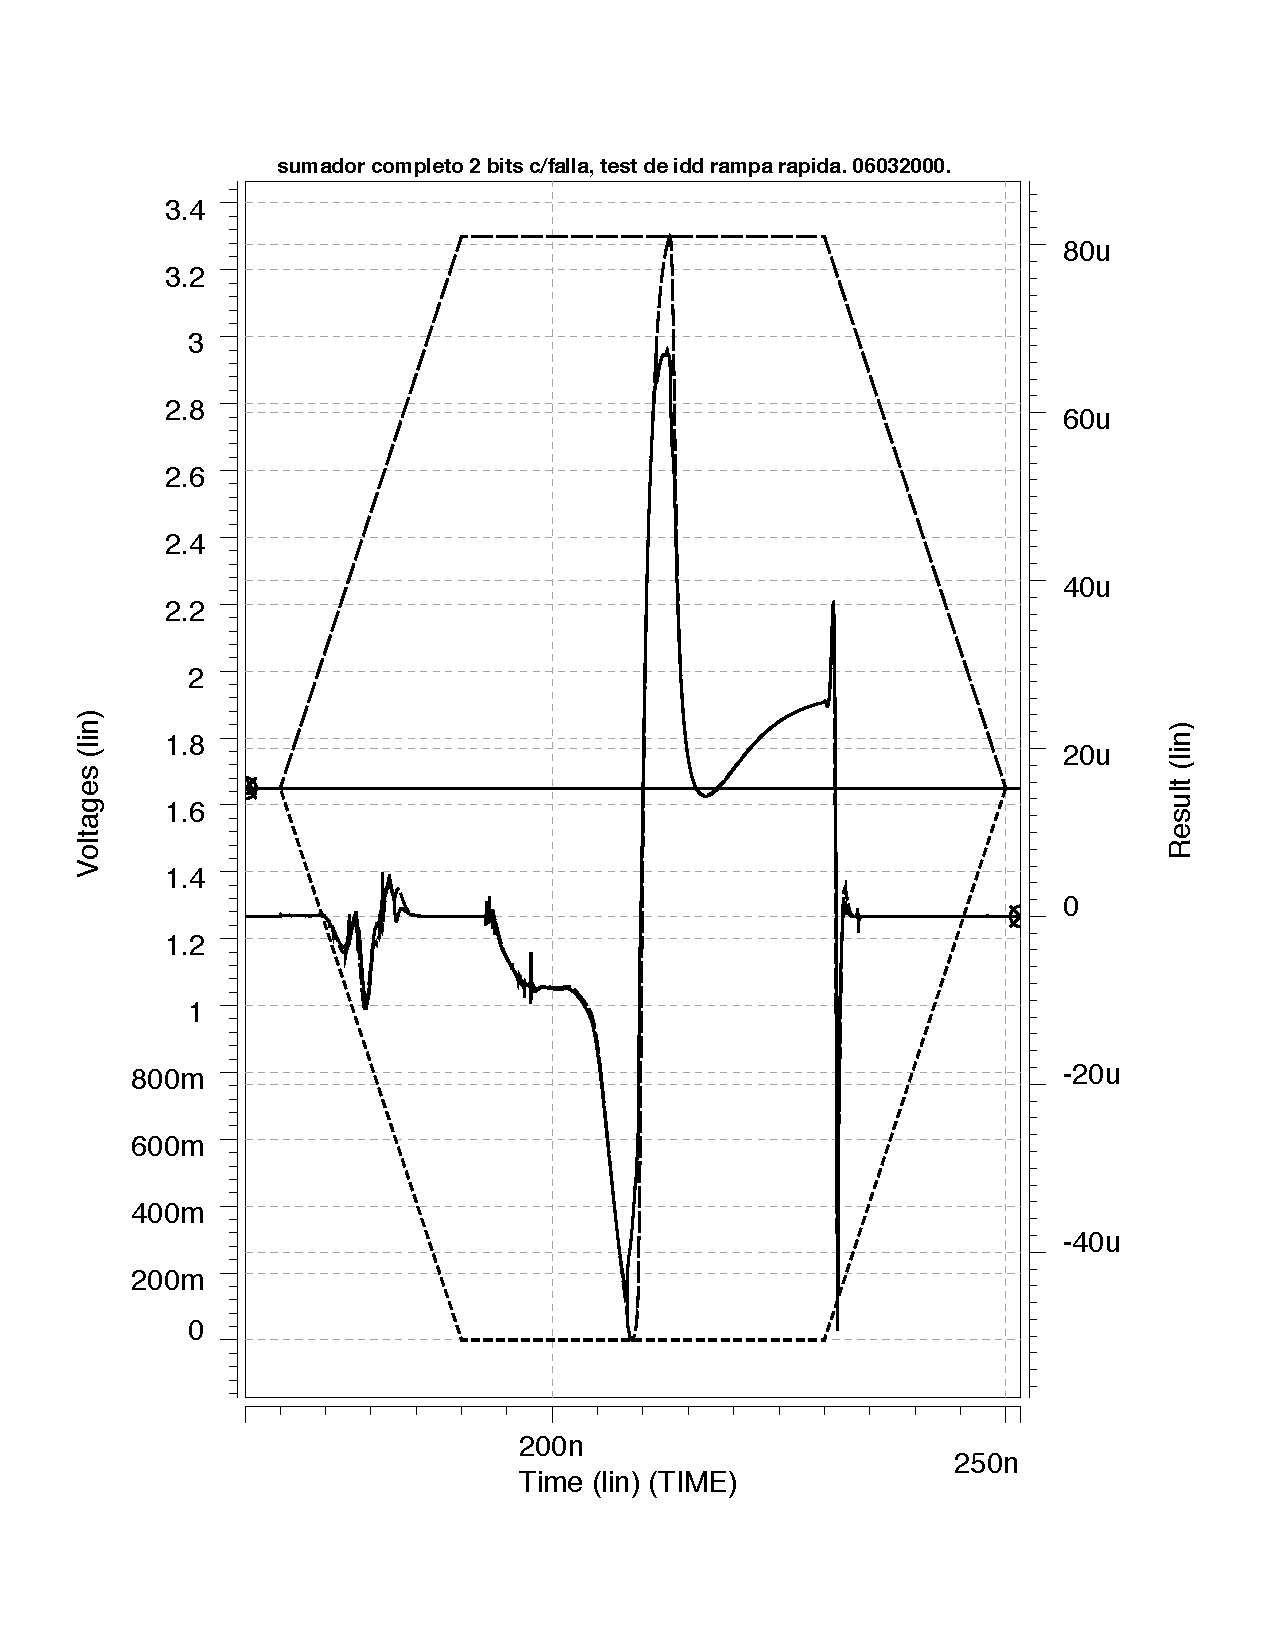
\includegraphics[width=0.32\linewidth]{rr50-4}&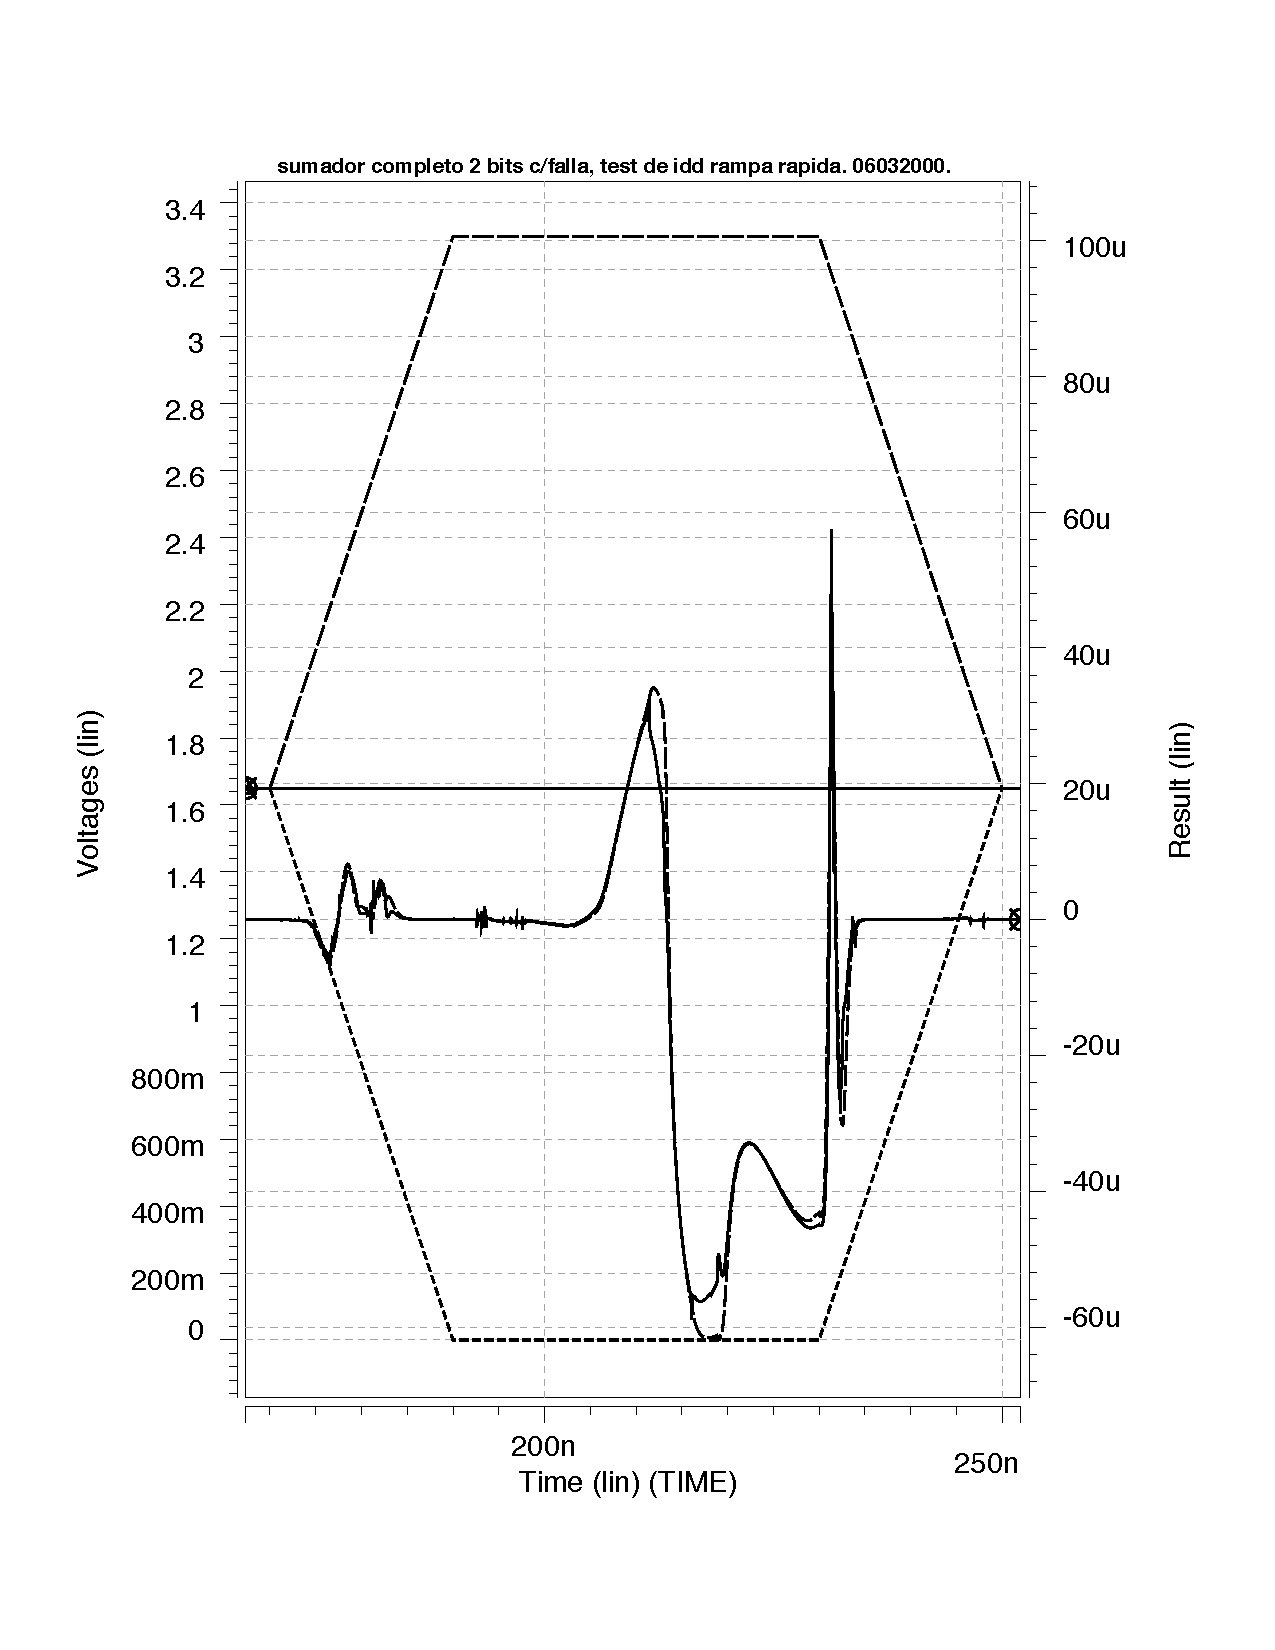
\includegraphics[width=0.32\linewidth]{rr60-6}\\
  \end{tabular}
  \label{tab:results}
\end{table}

\clearpage

\subsubsection{Resumen de fallas analizadas}
\label{sec:faultResume}

\begin{multicols}{2} % Divide text into multiple columns
\begin{itemize}
\item Fallas fáciles de detectar
  \begin{itemize}
  \item Fallas entre $V_{DD}$ ($V_{SS}$) y entradas
  \item Fallas entre nodos internos
  \item Fallas entre entradas y nodos internos
  \item La mayoría de las fallas entre $V_{DD}$ ($V_{SS}$) y nodos
    internos
  \end{itemize}
\item Fallas de detección difícil
  \begin{itemize}
  \item Fallas entre entradas
  \item Fallas entre nodos en los cuales existan transistores en
    paralelo
  \end{itemize}
\item Al variar la pendiente, se mejora la facilidad de detección de
fa\-llas entre alimentaciones y nodos internos
\item La zona estable del vector de prueba es importante para la detección.
\end{itemize}
\end{multicols}

\clearpage

\section{Conclusiones}
\label{sec:conclusion}

\begin{enumerate}
\item Se desarrolló un modelo de primer orden para predecir el
  comportamiento de las celdas CMOS estáticas en la aplicación de la
  prueba
\item Se desarrolló una optimización de tiempos de aplicación del
  vector de prueba para máxima detección
\item Se desarrolló una técnica que permite encontrar fallas de
  difícil detección
\item Según los resultados obtenidos se predice su aplicación en
  circuitos analógicos y mixtos
\end{enumerate}

Para mas información vea \cite{Mendoza2000}.

\clearpage

%----
% \begin{table}[ht]
% \caption{A table arranging  images}
% \centering
% \begin{tabular}{cc}
% \includegraphics[width=0.45\linewidth]{graphic1}&\includegraphics[width=0.45\linewidth]{graphic2}\\

% \includegraphics[width=0.45\linewidth]{graphic3}&\includegraphics[width=0.45\linewidth]{graphic4}\\
% \end{tabular}
% \label{tab:gt}
% \end{table}
%----

% \begin{table}[h]
% \centering
% \begin{tabular}{l l l}
% \toprule
% \textbf{Treatments} & \textbf{Response 1} & \textbf{Response 2}\\
% \midrule
% Treatment 1 & 0.0003262 & 0.562 \\
% Treatment 2 & 0.0015681 & 0.910 \\
% Treatment 3 & 0.0009271 & 0.296 \\
% \bottomrule
% \end{tabular}
% \caption{Table caption}
% \end{table}
%----

\thispagestyle{empty} % No slide header and footer

% \section{Mas información:}

\bibliographystyle{unsrt}
\bibliography{references}

\clearpage

%------------------------------------------------

% \thispagestyle{empty} % No slide header and footer

% \bibliographystyle{unsrt}
% \bibliography{references}

% \clearpage

%------------------------------------------------

\thispagestyle{empty} % No slide header and footer

\begin{tikzpicture}[remember picture,overlay] % Background box
\node [xshift=\paperwidth/2,yshift=\paperheight/2] at (current page.south west)[rectangle,fill,inner sep=0pt,minimum width=\paperwidth,minimum height=\paperheight/3,top color=mygreen,bottom color=mygreen]{}; % Change the height of the box, its colors and position on the page here
\end{tikzpicture}
% Text within the box
\begin{flushright}
\vspace{0.6cm}
\color{white}\sffamily
{\bfseries\LARGE ¿Preguntas?\par} % Request for questions text
\vfill
\end{flushright}

%----------------------------------------------------------------------------------------

\end{document}
